\chapter{Výsledky}
\label{7-vysledky}

Výsledky této práce jsou rozděleny do dvou částí podle analyzovaných dat -- na~analýzu časových řad souřadnic stanic systému \zkratka{DORIS} a~na~analýzu přesných drah družic vybavených přijímačem signálu systému \zkratka{DORIS}. Vzhledem k~objemu výsledků je v~hlavním textu uveden kompletní postup analýzy vždy na~jednom ukázkovém případu, který ilustruje celý analytický řetězec od~vstupních dat po~interpretaci. Pro~ostatní analyzované stanice a~družice jsou uvedeny pouze přehledy nalezených výsledků. Kompletní analýzy jsou obsaženy v~samostatných reportech tvořících přílohy této práce. Všechny grafy byly vytvořeny pomocí knihovny \texttt{matplotlib} v~jazyce Python.

\section{Časové řady}
\label{sec:casove-rady}

Analyzovány byly časové řady souřadnic stanic systému \zkratka{DORIS} za~období 2015 až 2025 s~využitím produktu STCD z~kumulativního řešení analytického centra GOP (verze gop25wd04), vzorkovaného s~týdenním krokem. Pro~analýzu byly vybrány stanice, jejichž chování bylo v~interním přehledu \zkratka{IDS} označeno jako podezřelé. U~stanic, kde v~analyzovaném období došlo k~výměně vysílače, je uveden identifikátor použitý pro analyzovanou časovou řadu:

\begin{itemize}
\item \textbf{KIVC} -- Kitab, Uzbekistán
\item \textbf{JIWC} -- Jiufeng, Čína
\item \textbf{LICB} -- Libreville, Gabon
\item \textbf{SARC} -- Sal, Kapverdy
\item \textbf{STKC} -- St.~John's, Kanada
\item \textbf{CADB} -- Cachoeira, Brazílie
\item \textbf{THUB} -- Thule, Grónsko
\item \textbf{MSPB} -- Mount Stromlo, Austrálie
\item \textbf{KRWB} -- Kourou, Francouzská Guyana
\end{itemize}

Cílem analýzy bylo indikované podezřelé chování potvrdit nebo vyvrátit, popsat jeho charakter a~pokusit se nalézt pravděpodobnou příčinu. Pro~každou stanici byl nejprve odhadnut lineární trend a~následně model s~jedním či více zlomy, který umožňuje zachytit skoky i~změny sklonu. Vhodnost jednotlivých modelů byla porovnána pomocí \zkratka{BIC}. Na~detrendovaných datech byla provedena spektrální analýza a~detekce diskontinuit dvěma nezávislými metodami. Výsledky byly ověřeny porovnáním s~blízkými stanicemi na~téže litosférické desce a~s~nezávislými kombinačními řešeními jiných analytických center.

V~následující části je podrobně popsán postup analýzy na~ukázkové stanici KIVC~-- Kitab, Uzbekistán. Tato stanice byla zvolena, protože je v~její časové řadě patrná změna trendu, skok i~periodická složka. Souhrnné výsledky pro~všechny analyzované stanice jsou uvedeny v~kapitole~\ref{sec:souhrn-casove-rady}, detailní analýzy jednotlivých stanic jsou obsaženy v~příloze.

\subsection{Ukázka analýzy: stanice KIVC~-- Kitab, Uzbekistán}

\subsubsection{Surová data}

Na obrázku~\ref{fig:kivc_raw} jsou znázorněny surové časové řady souřadnic stanice KIVC ve složkách dE, dN a dU za analyzované období.

\begin{figure}[H]
    \centering
    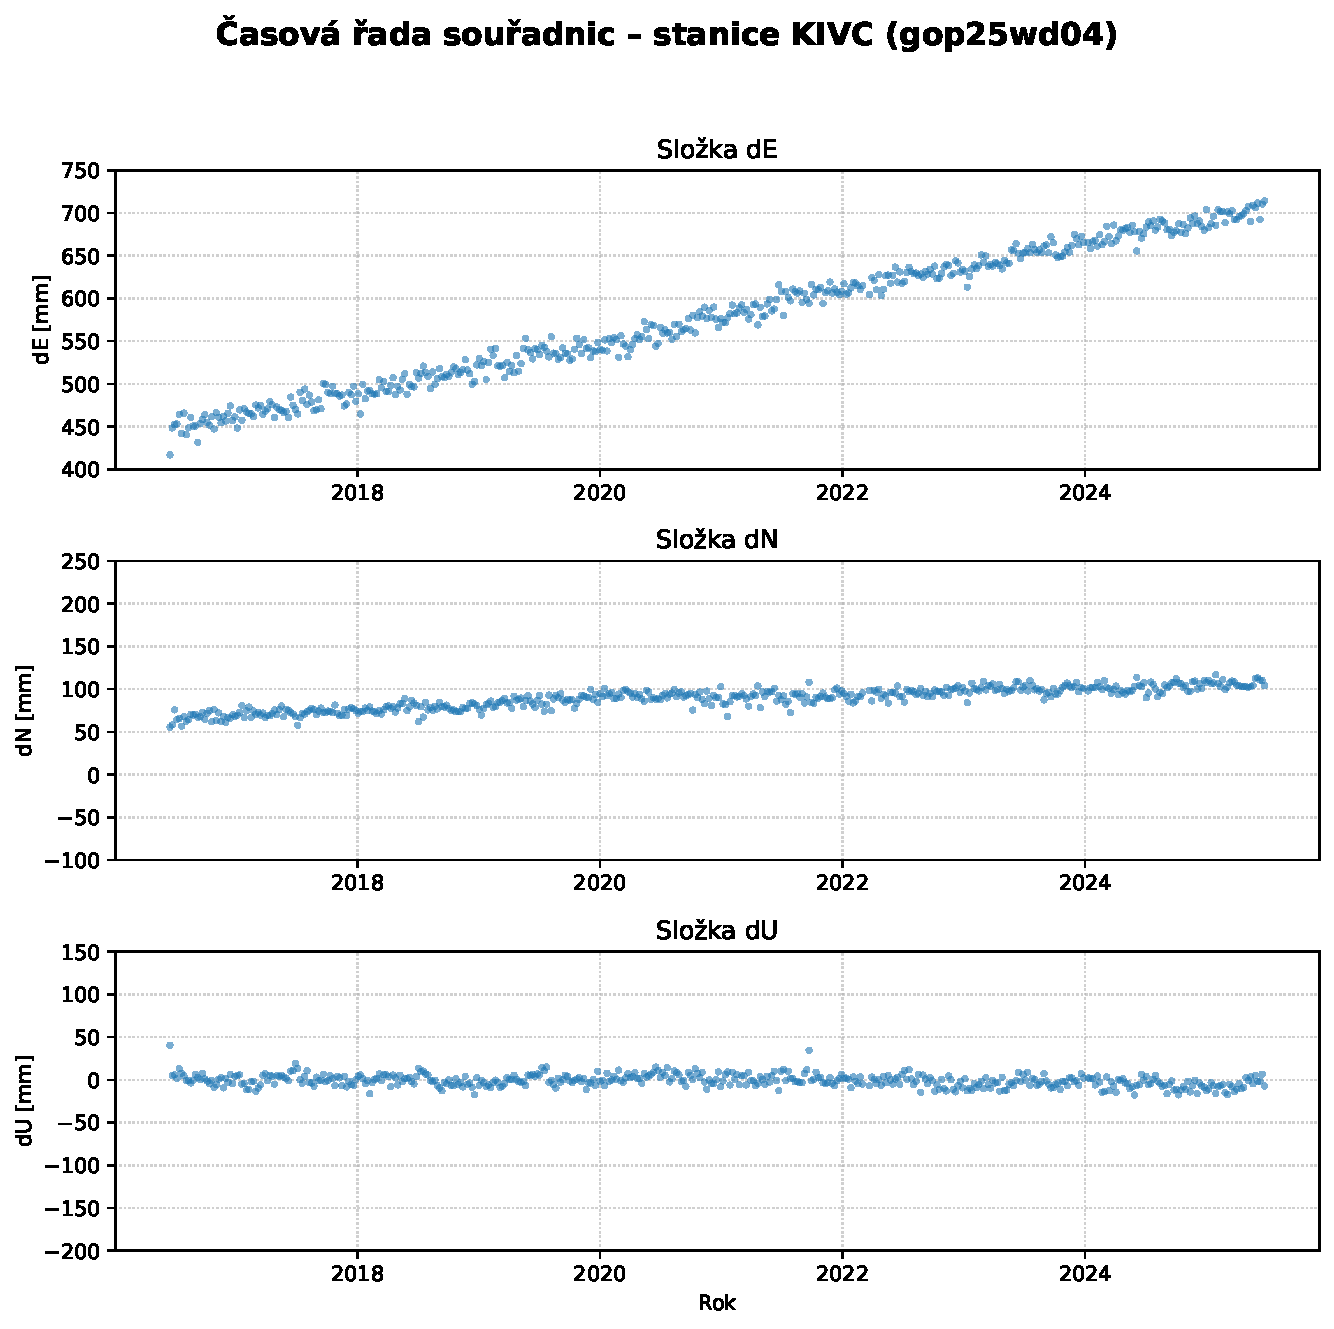
\includegraphics[width=1\textwidth]{images/results/stations/kivc/gop25wd04_stcd_kivc_raw_data.pdf}
    \caption{Surová časová řada souřadnic stanice KIVC (dE, dN, dU)}
    \label{fig:kivc_raw}
\end{figure}

\subsubsection{Lineární trend}

Na obrázku~\ref{fig:kivc_trend_1seg} je znázorněn vážený lineární trend časové řady souřadnic stanice KIVC, při jehož odhadu byly použity váhy \(p_i = 1/\sigma_i^2\). Z~výsledků je patrný výrazný lineární trend především ve složce dE, kde byla odhadnuta směrnice přibližně 29{,}1~mm/rok. Ve složce dN dosahuje trend přibližně 4{,}2~mm/rok a ve vertikální složce dU je trend mírně záporný, přibližně $-0{,}7$~mm/rok.

\begin{figure}[H]
    \centering
    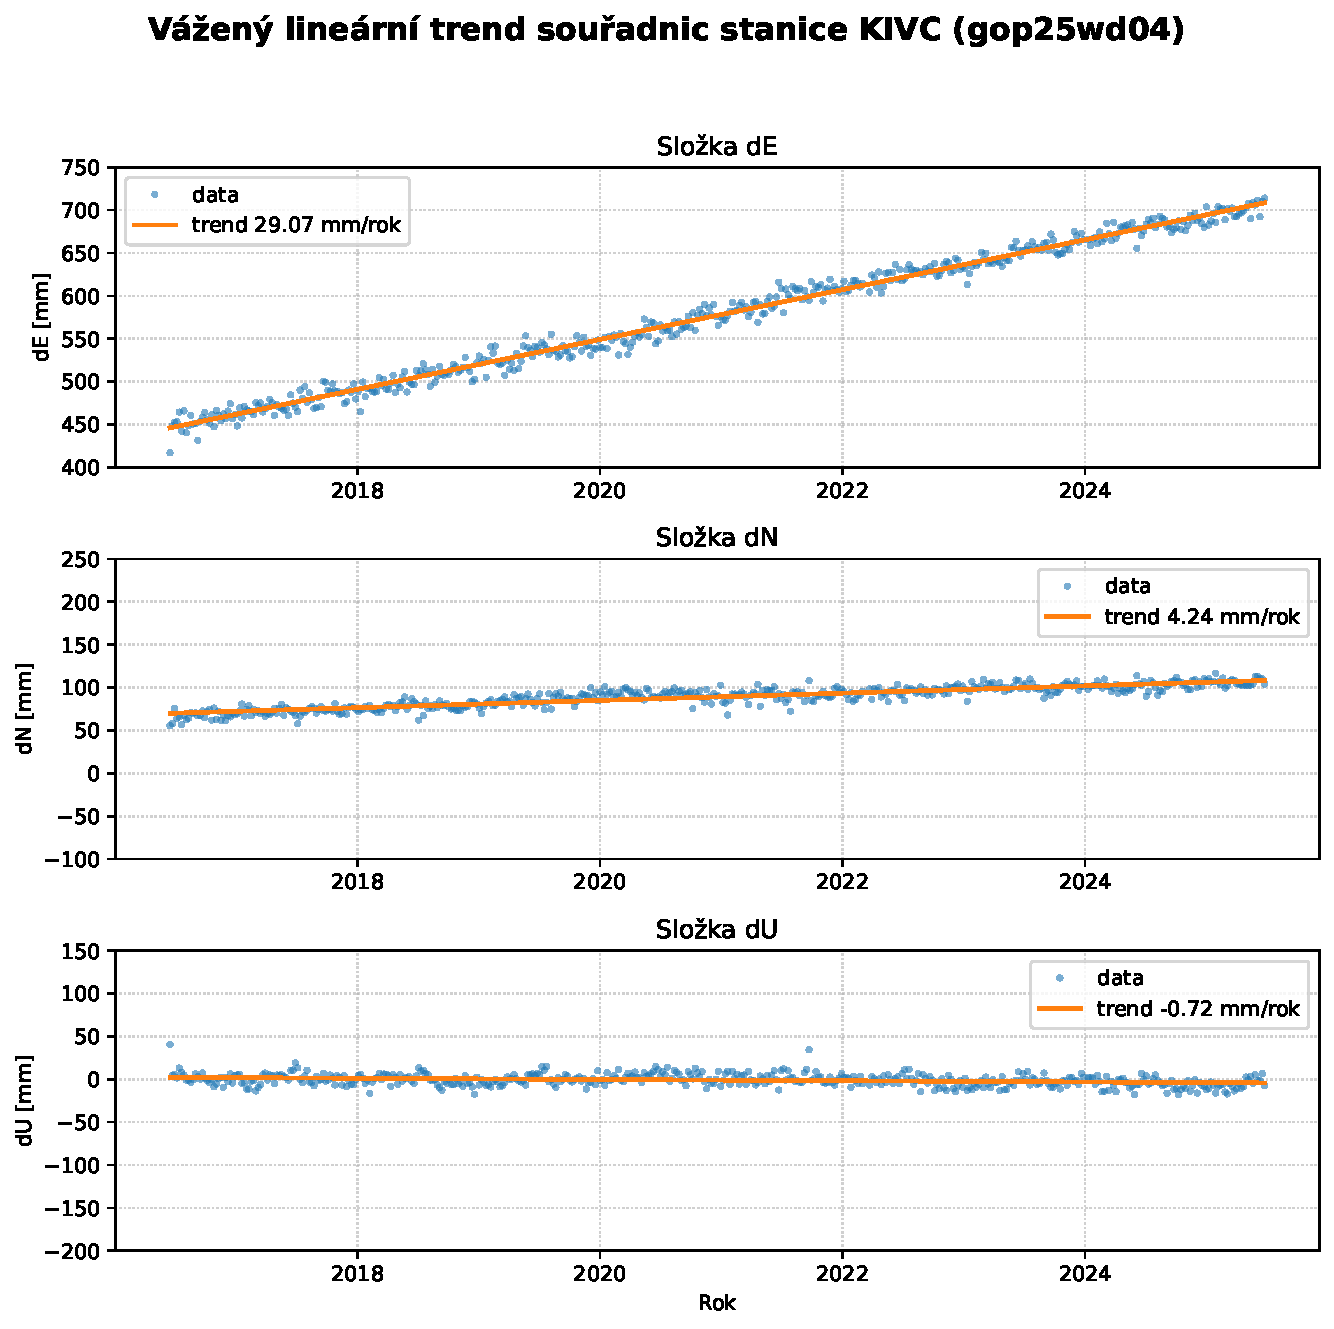
\includegraphics[width=1\textwidth]{images/results/stations/kivc/gop25wd04_stcd_kivc_trend_weighted_1seg.pdf}
    \caption{Vážený lineární trend souřadnic stanice KIVC}
    \label{fig:kivc_trend_1seg}
\end{figure}

Rezidua po odečtení lineárního trendu (obr.~\ref{fig:kivc_res_1seg}) naznačují přítomnost nenáhodných složek, což může znamenat, že lineární model není pro popis časové řady dostatečný.

\begin{figure}[H]
    \centering
    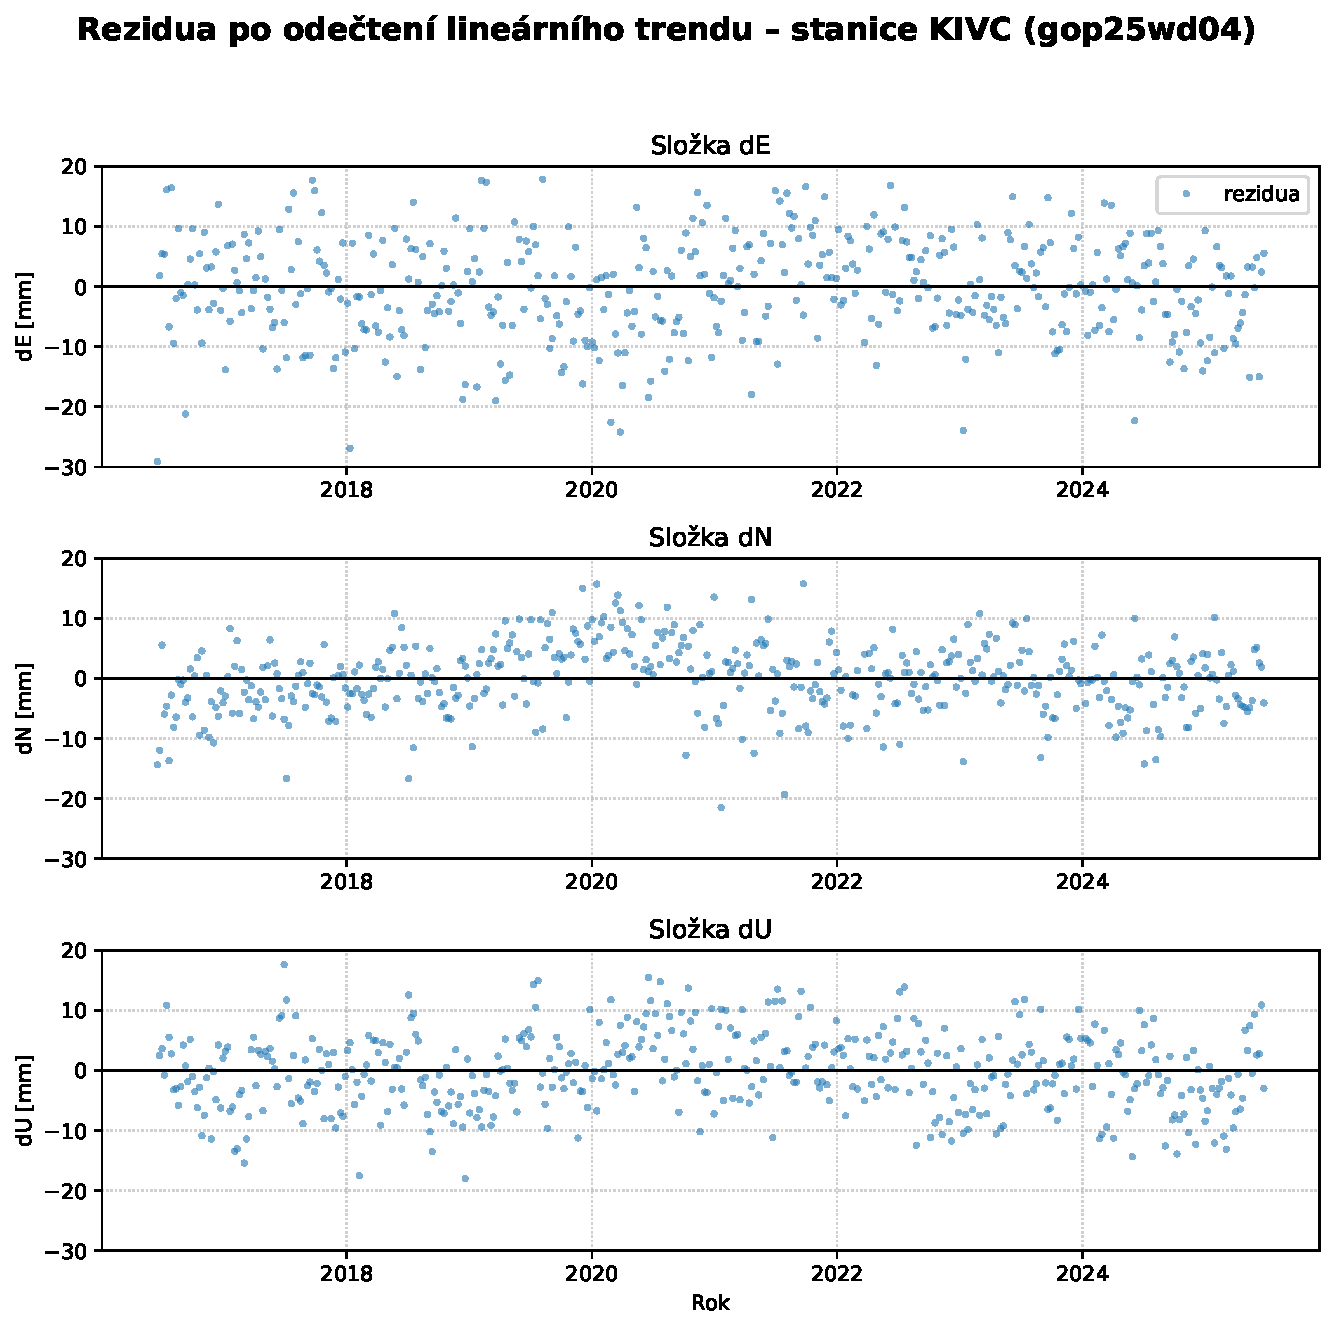
\includegraphics[width=1\textwidth]{images/results/stations/kivc/gop25wd04_stcd_kivc_residuals_weighted_1seg.pdf}
    \caption{Rezidua po odečtení lineárního trendu stanice KIVC}
    \label{fig:kivc_res_1seg}
\end{figure}

\subsubsection{Model se zlomy}

Pro zpřesnění popisu časové řady byl použit model se zlomy umožňující zachytit skoky a~změny trendu v~jednotlivých složkách souřadnic. Model byl odhadnut samostatně pro složky dE, dN a~dU, přičemž poloha
bodů zlomu byla určena iterativně na základě minimalizace hodnoty \zk{BIC}.

Na obrázku~\ref{fig:kivc_trend_breaks} je znázorněn výsledný model se zlomy a~v~tabulce~\ref{tab:gop25wd04_stcd_kivc_trend_weighted_multiseg} jsou shrnuty identifikované body zlomu včetně odhadnutých velikostí skoků a~změn trendu.

\begin{figure}[H]
    \centering
    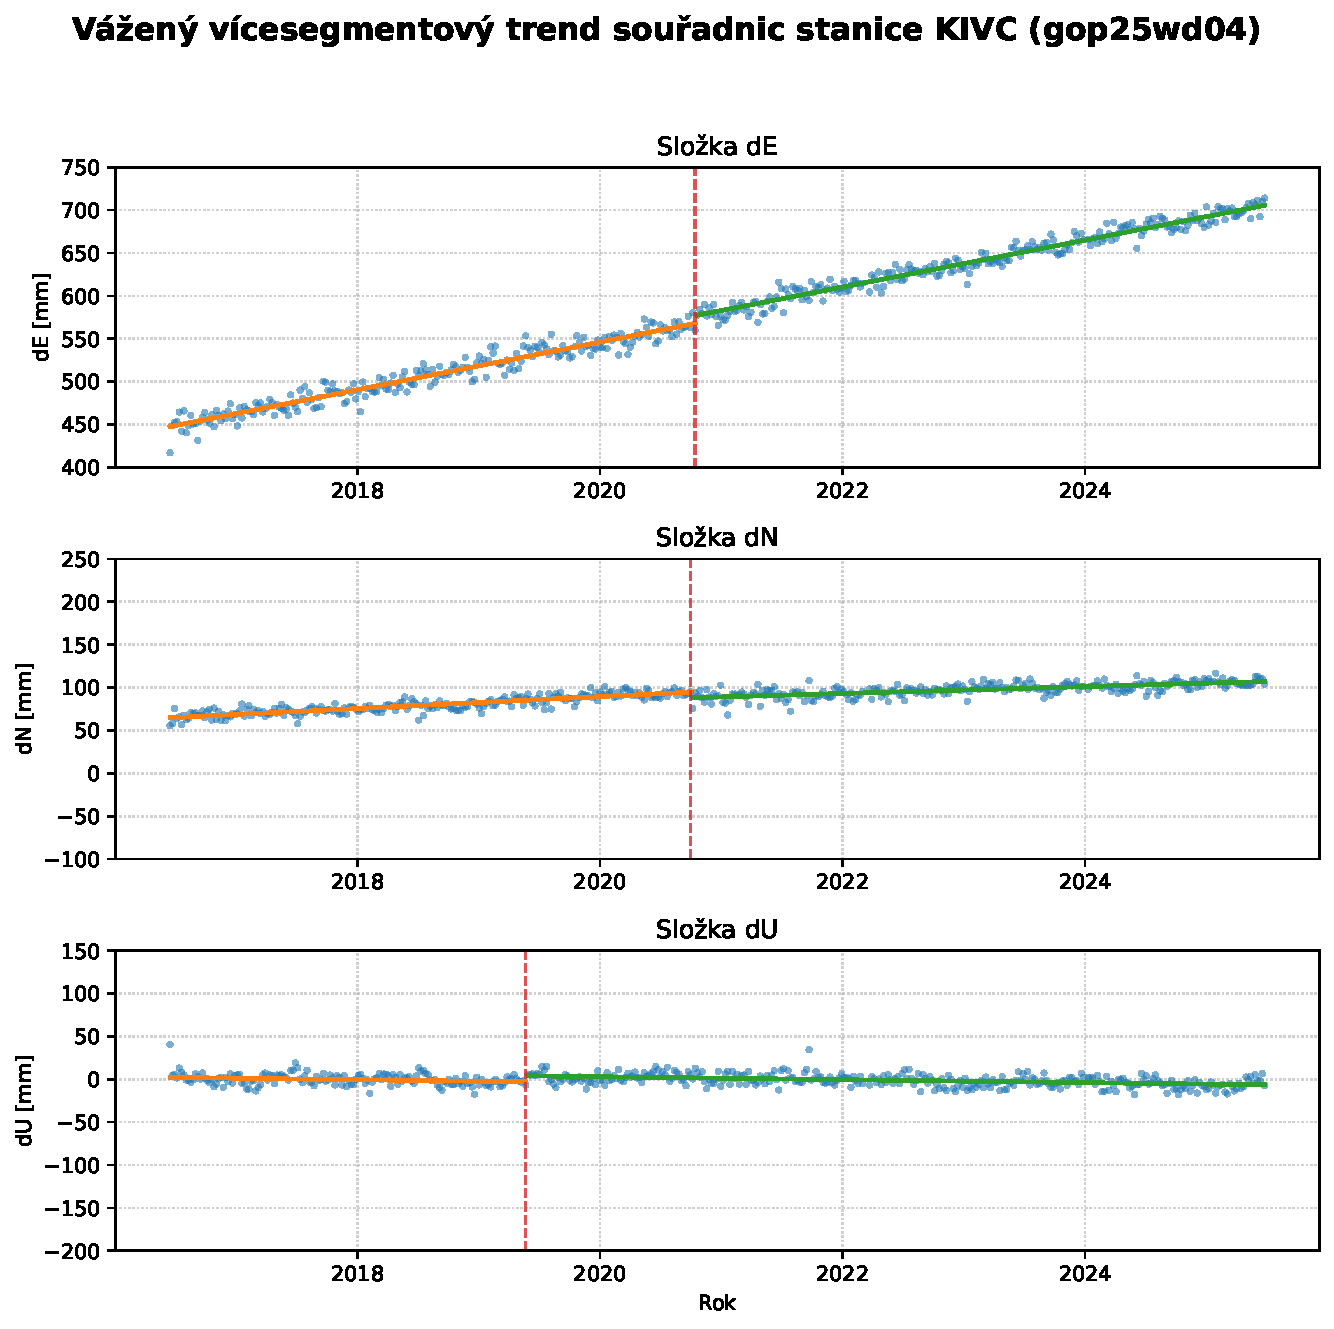
\includegraphics[width=1\textwidth]{images/results/stations/kivc/gop25wd04_stcd_kivc_trend_weighted_multiseg.pdf}
    \caption{Vážený model se zlomy pro souřadnice stanice KIVC}
    \label{fig:kivc_trend_breaks}
\end{figure}

\begin{table}[H]
\centering
\small
\caption{Identifikované zlomy v~časové řadě stanice KIVC.}
\label{tab:gop25wd04_stcd_kivc_trend_weighted_multiseg}
\begin{tabular}{lllllr}
\toprule
Složka & Počet segmentů & Zlomy & Trendy [mm/rok] & Skoky [mm] & $R^2$ \\
\midrule
dE & 2 & 14. 10. 2020 & 27.796, 27.359 & 9.125 & 0.989 \\
dN & 2 & 29. 9. 2020 & 6.952, 3.999 & -6.560 & 0.828 \\
dU & 2 & 22. 5. 2019 & -1.782, -1.725 & 7.062 & 0.166 \\
\bottomrule
\end{tabular}
\end{table}


Ve složkách dE a~dN byly identifikovány zlomy v~druhé polovině roku 2020. Ve složce dU byl nalezen dřívější zlom v~roce 2019. Zatímco ve složce dE se trend po zlomu změnil jen nepatrně, ve složce dN se trend změnil zhruba o~3~mm/rok.

Použití modelu se zlomy vede k~potlačení nenáhodného charakteru reziduí, jak je patrné z~obrázku~\ref{fig:kivc_res_breaks}. Snížení hodnot \zk{RMS} reziduí je uvedeno v~tabulce~\ref{tab:gop25wd04_stcd_kivc_residual_rms_comparison}.

\begin{table}[H]
\centering
\small
\caption{Porovnání RMS reziduí pro stanici KIVC}
\label{tab:gop25wd04_stcd_kivc_residual_rms_comparison}
\begin{tabular}{lrrr}
\toprule
Složka & Lineární [mm] & Se zlomy [mm] & Snížení [\%] \\
\midrule
dE & 8.45 & 8.15 & 3.5 \\
dN & 5.78 & 5.24 & 9.3 \\
dU & 6.75 & 6.46 & 4.4 \\
\bottomrule
\end{tabular}
\end{table}


\begin{figure}[H]
    \centering
    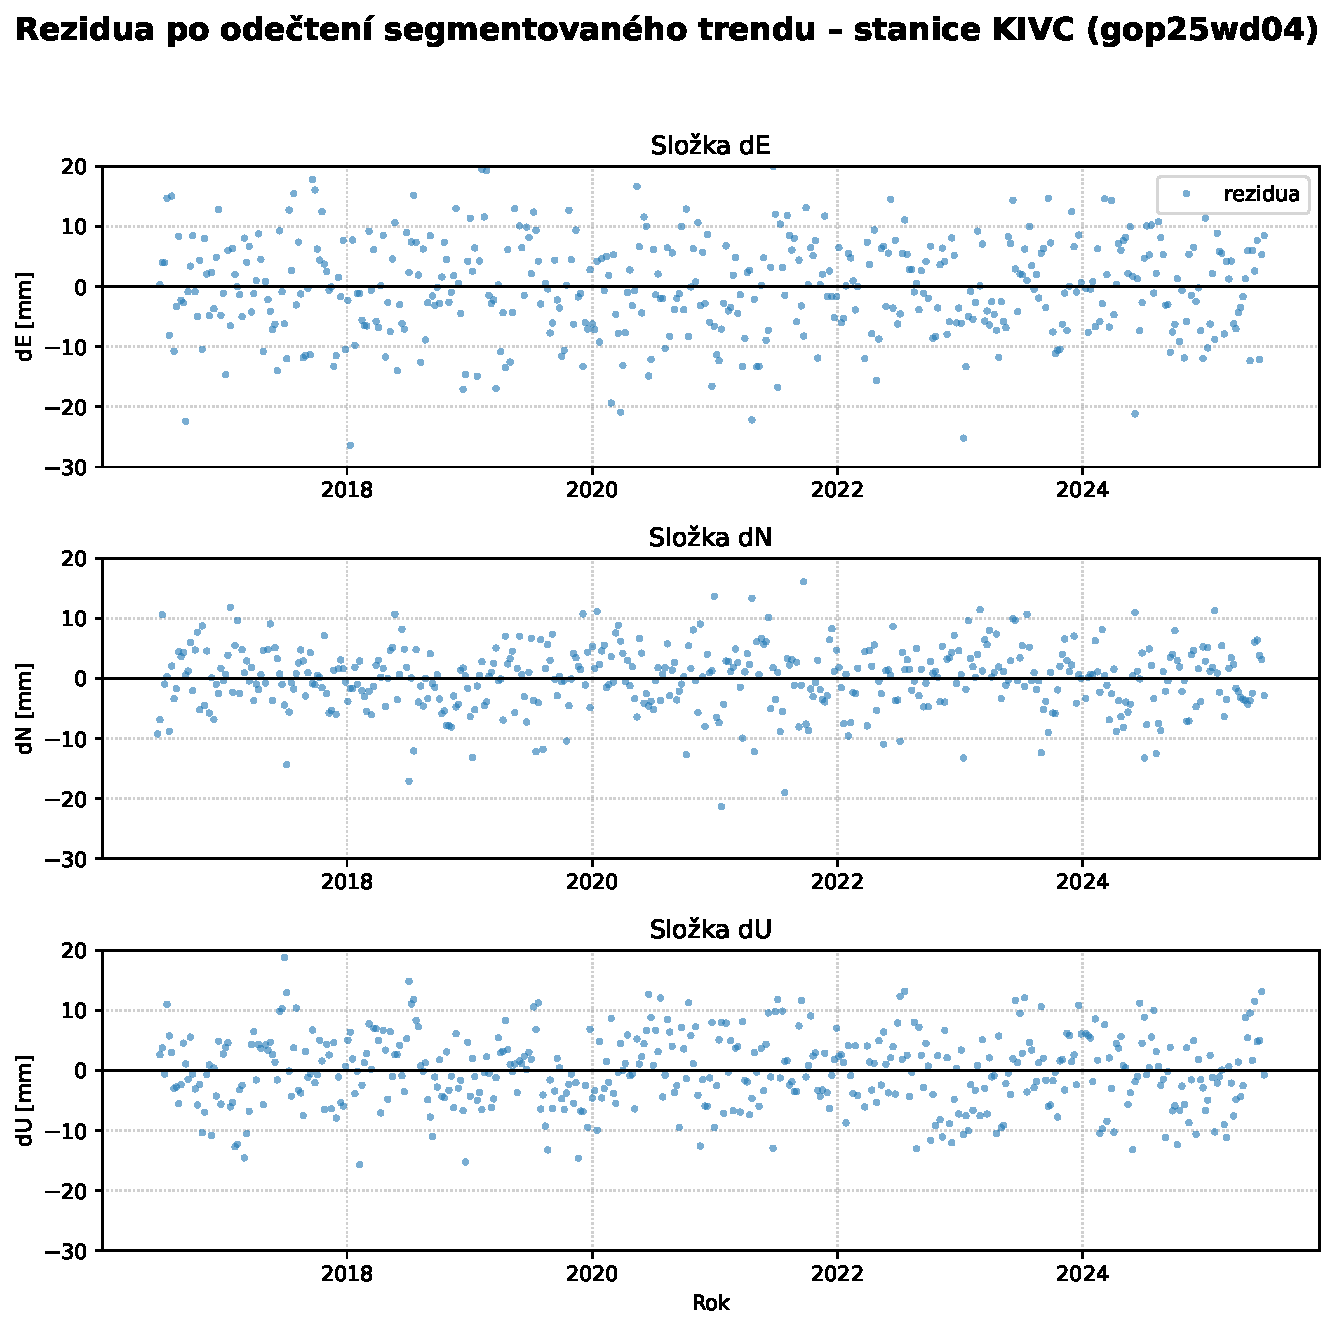
\includegraphics[width=1\textwidth]{images/results/stations/kivc/gop25wd04_stcd_kivc_residuals_weighted_multiseg.pdf}
    \caption{Rezidua po odečtení modelu se zlomy stanice KIVC}
    \label{fig:kivc_res_breaks}
\end{figure}

\subsubsection{Detekce diskontinuit}

Detekce diskontinuit byla provedena na reziduích po odečtení jednoduchého lineárního trendu, tedy před aplikací modelu se zlomy. Cílem bylo nezávisle ověřit, zda se v~časové řadě projeví diskontinuity naznačené modelem se zlomy. Použity byly dvě nezávislé metody: metoda dvou pohyblivých oken (obr.~\ref{fig:kivc_sliding_window}) a~metoda založená na analýze derivace vyhlazené časové řady (obr.~\ref{fig:kivc_lowess_derivative}).

\begin{figure}[H]
    \centering
    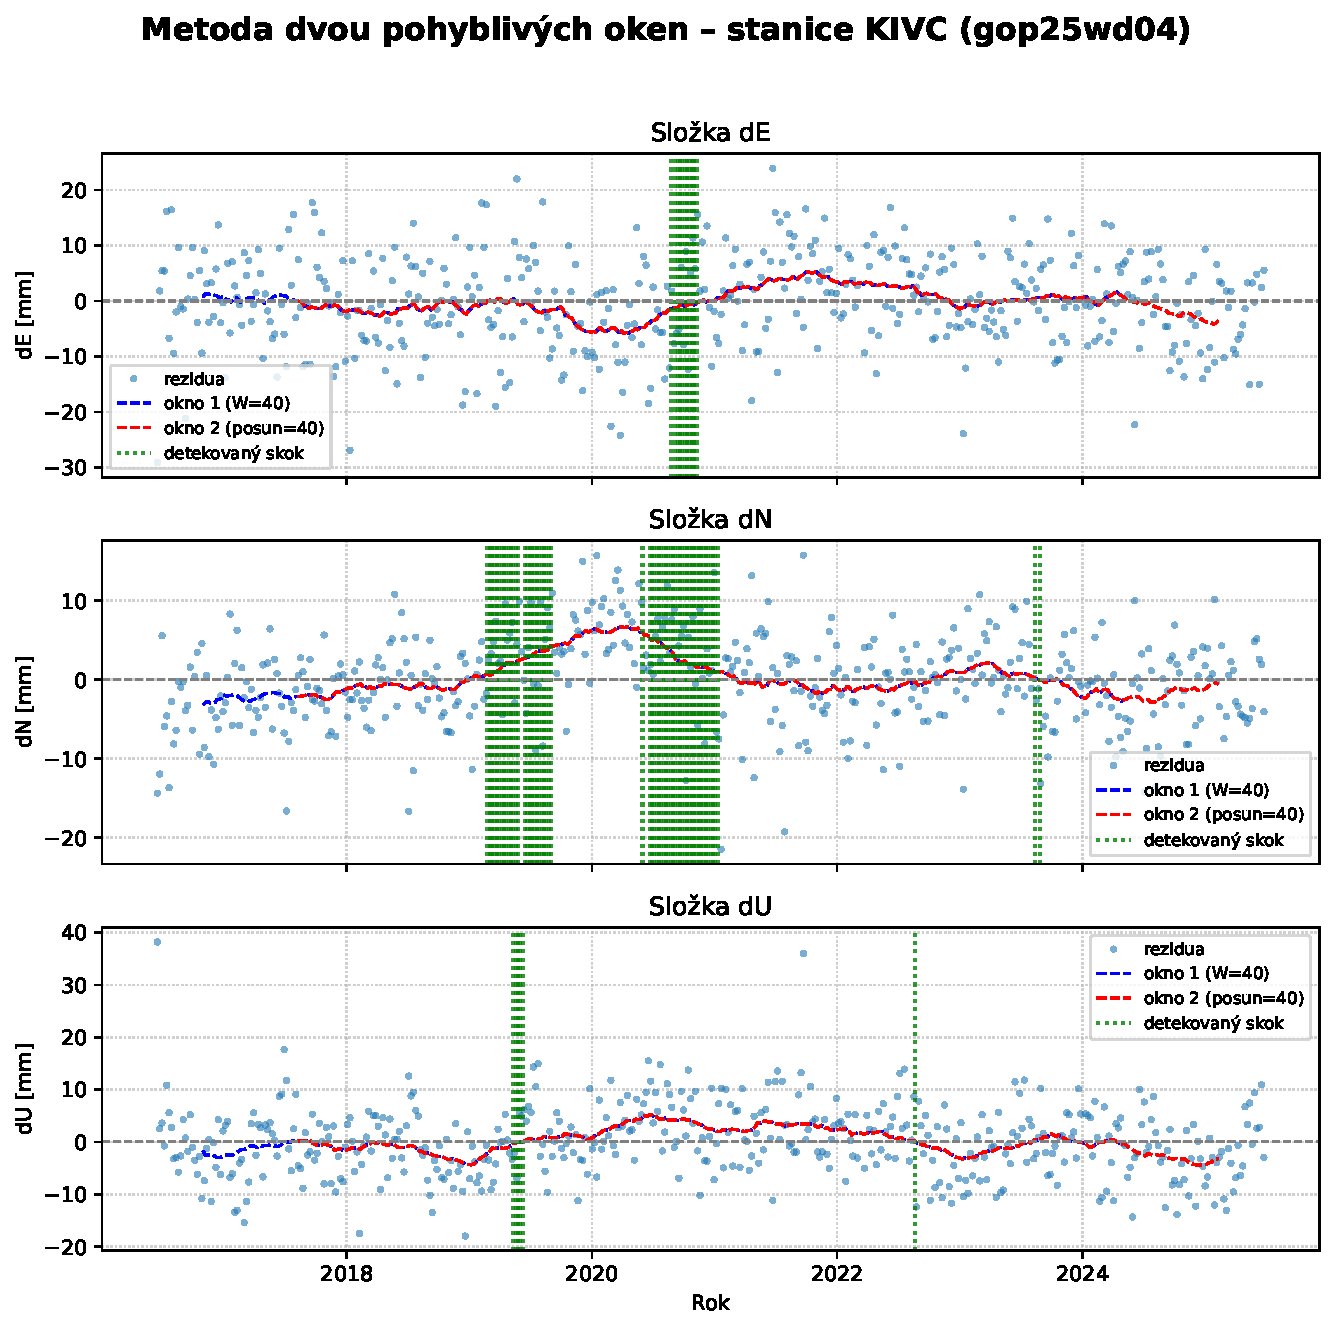
\includegraphics[width=1\textwidth]{images/results/stations/kivc/gop25wd04_stcd_kivc_detr_weighted_1seg_sliding_window.pdf}
    \caption{Detekce diskontinuit stanice KIVC pomocí dvou pohyblivých oken}
    \label{fig:kivc_sliding_window}
\end{figure}

\begin{figure}[H]
    \centering
    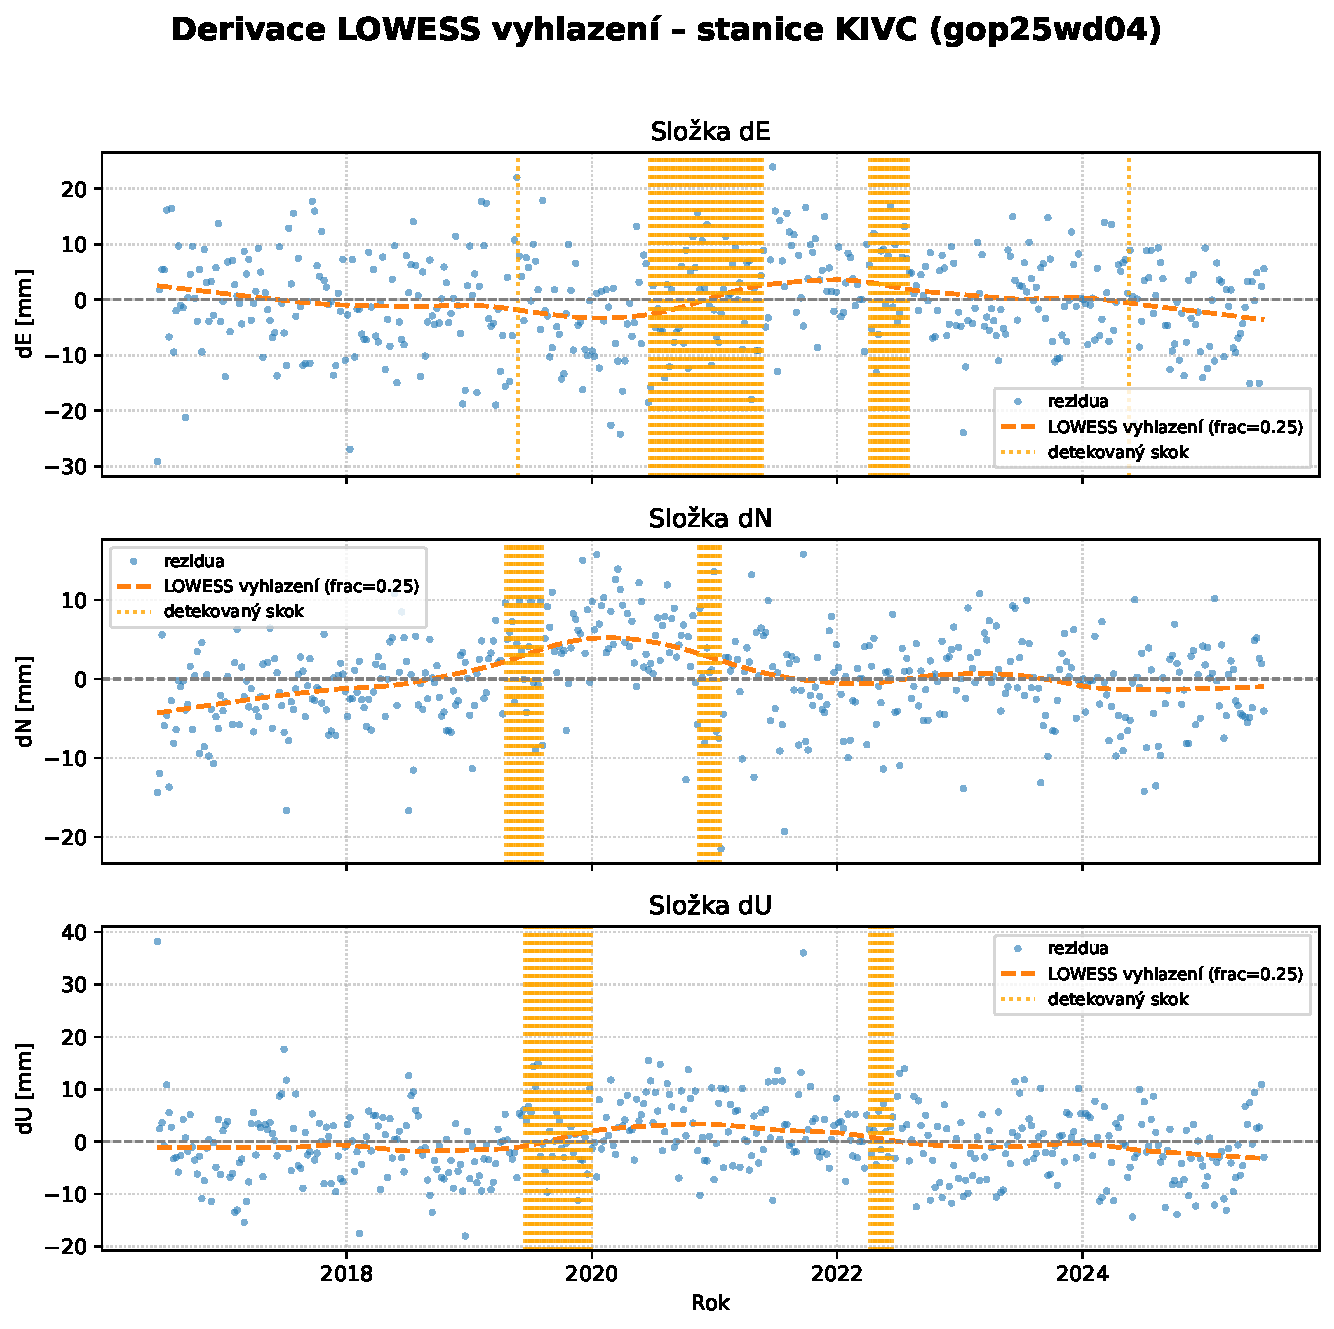
\includegraphics[width=1\textwidth]{images/results/stations/kivc/gop25wd04_stcd_kivc_detr_weighted_1seg_lowess_derivate.pdf}
    \caption{Detekce diskontinuit stanice KIVC pomocí analýzy derivace}
    \label{fig:kivc_lowess_derivative}
\end{figure}

Obě metody potvrzují, že časová řada stanice KIVC neobsahuje pouze náhodný rozptyl kolem lineárního trendu, ale také změny odpovídající diskontinuitám. Nejvýraznější shoda s~modelem se zlomy je patrná v~období kolem roku 2020, zejména v~horizontálních složkách dE a~dN. Ve složce dU jsou detekce méně jednoznačné.

\subsubsection{Spektrální analýza}

Spektrální analýza byla provedena na reziduích po odečtení lineárního trendu. Cílem bylo ověřit, zda nenáhodný charakter reziduí může být vysvětlen dominantní periodickou složkou. Na obrázku~\ref{fig:kivc_fft_periodogram} je uveden amplitudový periodogram získaný pomocí algoritmu \zkratka{FFT}.

\begin{figure}[H]
    \centering
    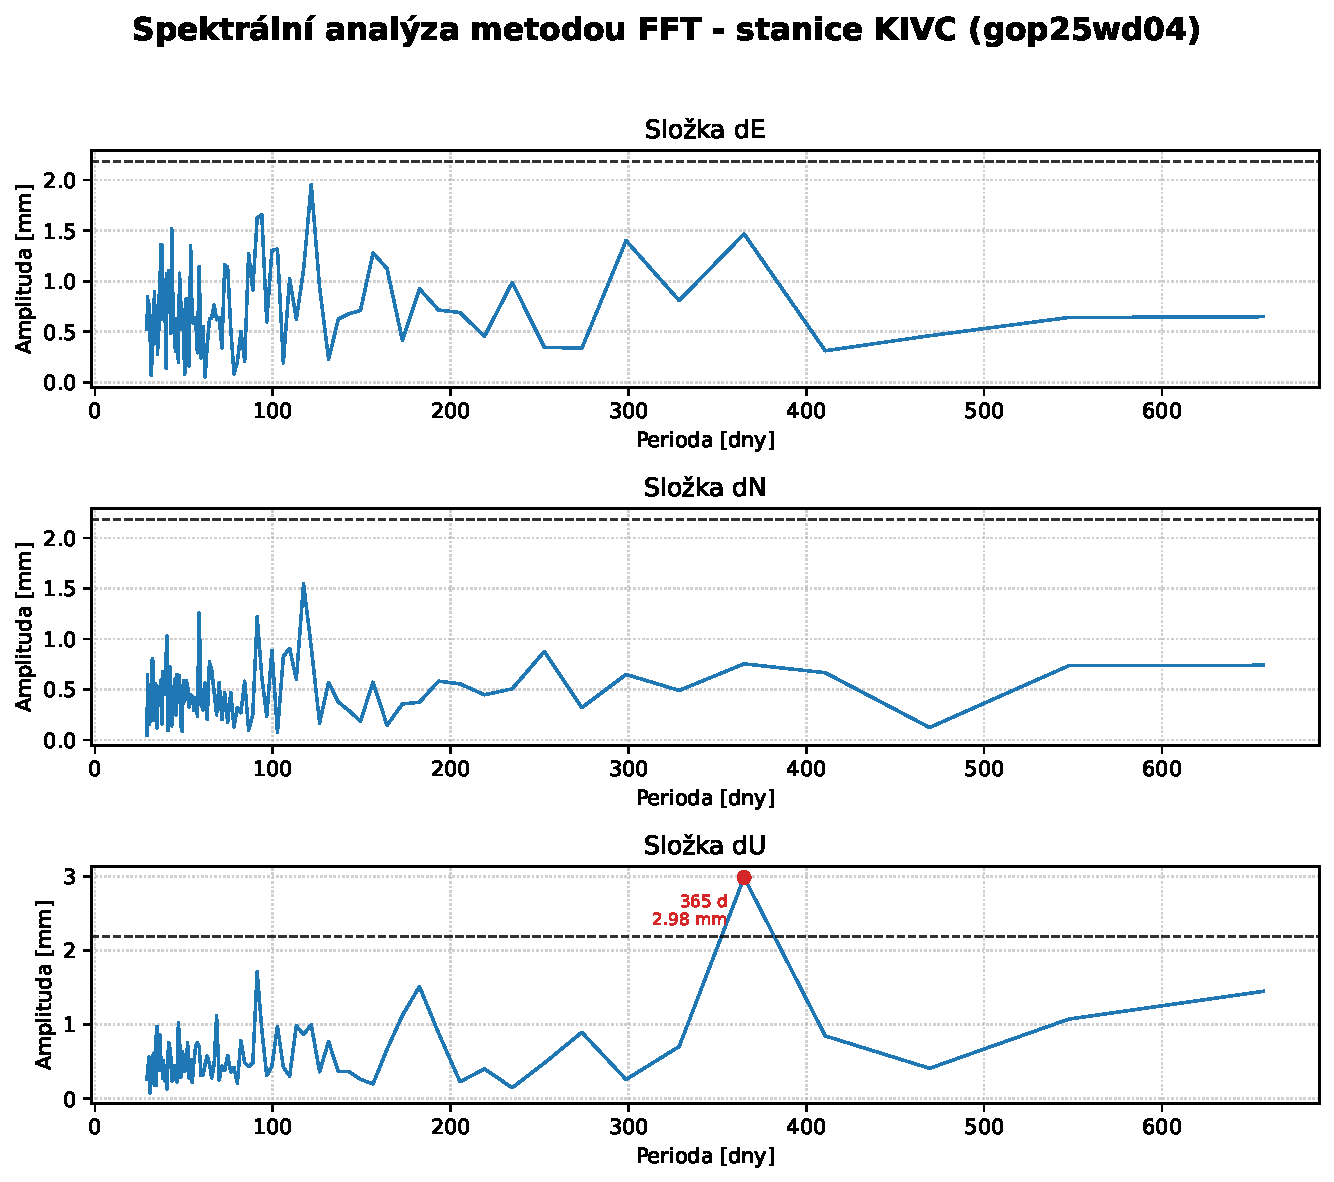
\includegraphics[width=1\textwidth]{images/results/stations/kivc/gop25wd04_stcd_kivc_detr_weighted_1seg_spectral_fft_periodogram.pdf}
    \caption{Periodogram reziduí stanice KIVC po odečtení lineárního trendu}
    \label{fig:kivc_fft_periodogram}
\end{figure}

Významná periodicita byla nalezena pouze ve vertikální složce dU, a to pro periodu přibližně 365~dní s~amplitudou přibližně 3{,}0~mm. Ve vodorovných složkách dE a~dN nebyla identifikována výrazná periodická složka.

Na základě nalezené periodicity byla rekonstruována periodická složka časové řady. Její průběh je znázorněn na obrázku~\ref{fig:kivc_fft_periodic_component}.

\begin{figure}[H]
    \centering
    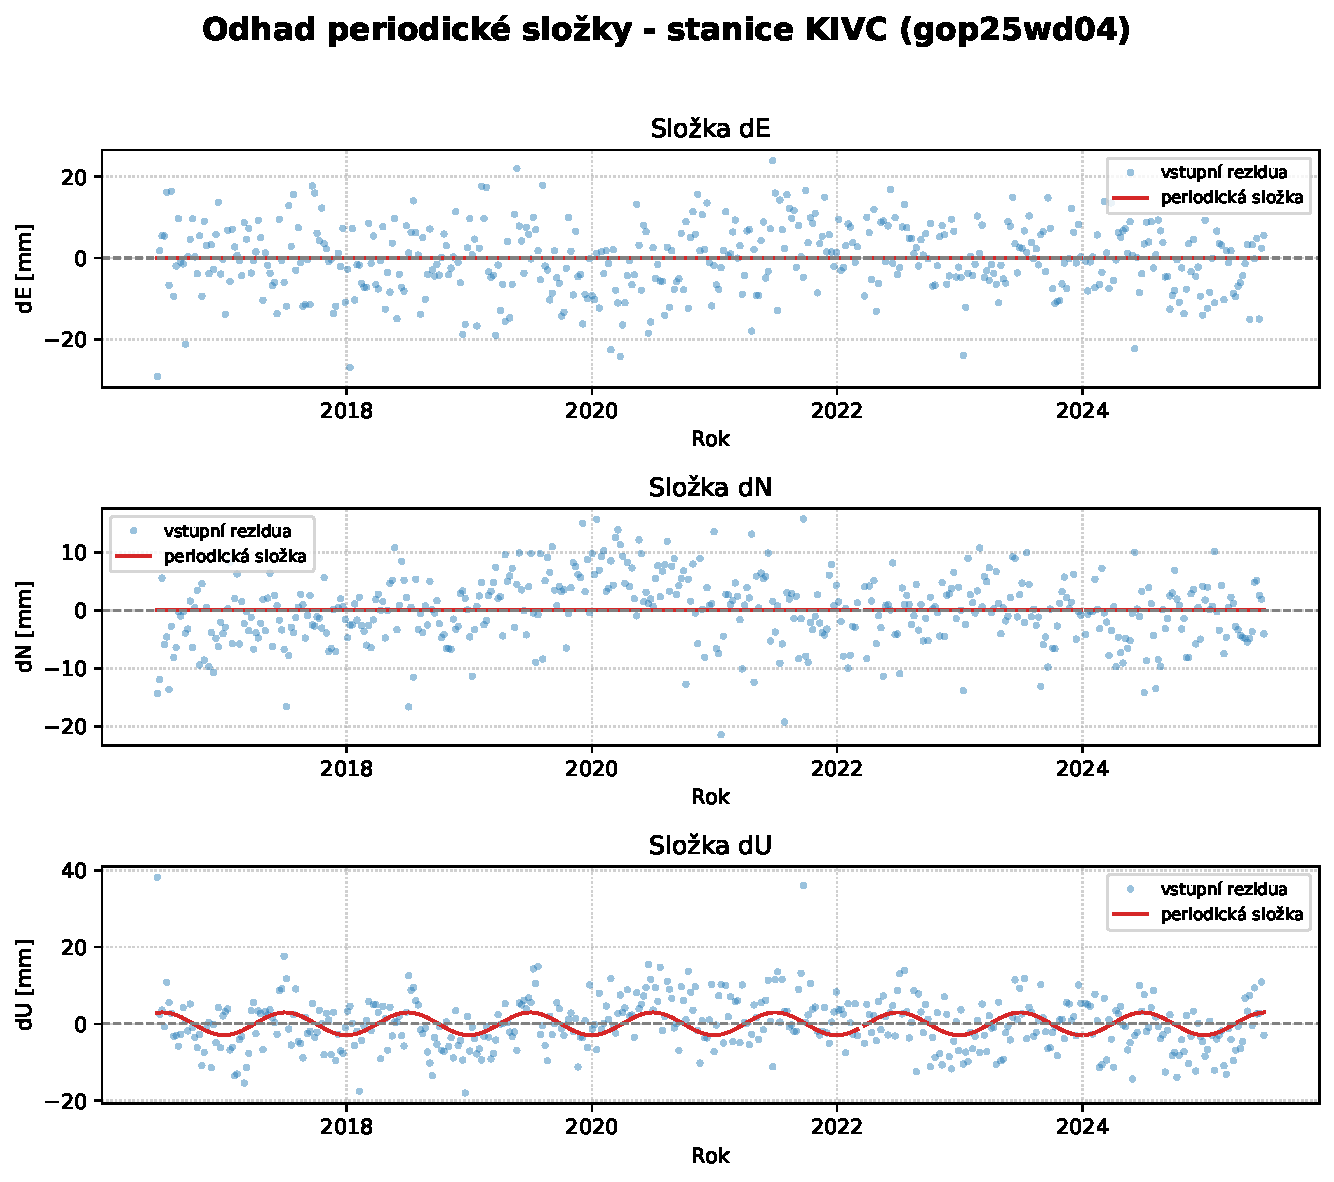
\includegraphics[width=\textwidth]{images/results/stations/kivc/gop25wd04_stcd_kivc_detr_weighted_1seg_spectral_fft_periodic_component.pdf}
    \caption{Rekonstruovaná periodická složka reziduí stanice KIVC}
    \label{fig:kivc_fft_periodic_component}
\end{figure}

Vliv odečtení periodické složky na rozptyl reziduí je uveden v~tabulce~\ref{tab:gop25wd04_stcd_kivc_detr_weighted_1seg_spectral_fft_variance_reduction}.

\begin{table}[htbp]
\caption{Snížení rozptylu po odstranění významných periodických složek určených metodou FFT pro stanici KIVC a řešení gop25wd04.}
\label{tab:gop25wd04_stcd_kivc_detr_weighted_1seg_spectral_fft_variance_reduction}
\begin{tabular}{llrrrr}
\toprule
Složka & Počet period & Rozptyl před [mm$^2$] & Rozptyl po [mm$^2$] & Snížení [mm$^2$] & Snížení [\%] \\
\midrule
dE & 0 & 71.396 & 71.396 & 0.000 & 0.0 \\
dN & 0 & 33.442 & 33.442 & 0.000 & 0.0 \\
dU & 1 & 45.664 & 41.221 & 4.443 & 9.7 \\
\bottomrule
\end{tabular}
\end{table}


Po odečtení roční periodické složky došlo ke snížení rozptylu vertikálních reziduí přibližně o~9{,}7~\%.

\subsubsection{Porovnání s~blízkými stanicemi}

Pro ověření, zda zjištěné změny mohou mít regionální charakter, byla stanice KIVC porovnána s~blízkými stanicemi ležícími na stejné litosférické desce. V~požadovaném časovém rozsahu byla dostupná stanice EVEB. Její časová řada vykazuje ve složkách dE a dN obdobné chování jako stanice KIVC, ve složce dU je výraznější periodická složka.

\subsubsection{Porovnání s~nezávislými řešeními}

Výsledky byly dále porovnány s~nezávislými kombinačními řešeními GRG, ESA a~GSC. Tato řešení vykazují podobné dlouhodobé chování časové řady, identické diskontinuity jako v~řešení GOP se však v~ostatních řešeních nevyskytují. Přesné epochy a velikosti diskontinuit se mezi řešeními liší a identické diskontinuity jako v~řešení GOP se v~ostatních řešeních nevyskytují.

\subsubsection{Interpretace}

Analýza stanice KIVC potvrzuje podezřelé chování indikované v~přehledu IDS, zejména změny ve vodorovných složkách kolem roku 2020. Ve složce dE byl nalezen skok přibližně $9{,}1$~mm bez výrazné změny trendu. Ve složce dN byl nalezen skok přibližně $-6{,}6$~mm a změna trendu přibližně o~3~mm/rok. Ve složce dU byl nalezen skok přibližně 7~mm v~roce 2019 bez výrazné změny trendu. Roční periodicita byla nalezena pouze ve vertikální složce a s~podezřelým chováním stanice zřejmě nemá přímou souvislost. Obdobné chování bylo částečně pozorováno také u~blízké stanice EVEB. Přímou souvislost se seismickou aktivitou ani s~přechodem z~\texttt{GOP67} na \texttt{GOP70} se nepodařilo prokázat.

\subsection{Souhrnné výsledky}
\label{sec:souhrn-casove-rady}

V~této části jsou shrnuty hlavní závěry analýzy všech vybraných stanic. Uvedeny jsou pouze výsledky, které mají význam pro interpretaci podezřelého chování stanic. Kompletní grafické výstupy, odhady trendů, detekce diskontinuit a porovnání s~nezávislými řešeními jsou uvedeny v~příloze~report\_stations.pdf.

\subsubsection{KIVC -- Kitab, Uzbekistán}

U~stanice KIVC bylo potvrzeno podezřelé chování indikované na přelomu let 2019 a 2020. Nejvýrazněji se projevilo ve vodorovných složkách, kde byl ve složce dE identifikován skok přibližně $9{,}1$~mm a ve složce dN skok přibližně \(-6{,}6\)~mm doprovázený změnou trendu přibližně o~3~mm/rok. Ve vertikální složce dU byl nalezen skok přibližně 7~mm v~roce 2019. Obdobné chování bylo pozorováno také u~blízké stanice EVEB, zatímco v~nezávislých řešeních GRG, ESA a GSC se identické diskontinuity nevyskytují. Příčinu se nepodařilo jedno\-značně určit. Seismická aktivita ani přechod z~\texttt{GOP67} na \texttt{GOP70} nebyly potvrzeny jako pravděpodobné vysvětlení.

\subsubsection{JIWC -- Jiufeng, Čína}

U~stanice JIWC se podezřelé chování projevuje především ve vertikální složce dU po roce 2020. Po přerušení časové řady v~roce 2019 se rezidua ve složce dU výrazně rozptylují a průběh časové řady se spíše pozvolna vlní, než že by obsahoval jeden jednoznačný skok. Podobný charakter má tato složka také v~nezávislých řešeních GRG, ESA a GSC, takže se pravděpodobně nejedná pouze o~artefakt řešení GOP. Jednoznačnou příčinu se nepodařilo určit. Seismická aktivita ani zjištěné periodické složky pozorované chování dostatečně nevysvětlují.

\subsubsection{LICB -- Libreville, Gabon}

U~stanice LICB byl ve složce dU nalezen v~roce 2016 skok přibližně $18{,}9$~mm. Ve složkách dE a~dN byly identifikovány také další diskontinuity a ve složce dE byly nalezeny výrazné periodické složky, včetně periody přibližně $118$~dní odpovídající beta-prime periodě družic typu Jason a~Sentinel-6A. Blízké stanice HEMB a~SARC obdobné chování v~okolí roku~2016 nevykazují. Řešení ESA vykazuje podobné nestandardní chování jako řešení GOP, zatímco řešení GRG a~GSC se v~nalezených diskontinuitách a periodicitách liší, vykazují však také určité nestandardní chování. Vzhledem k~časové blízkosti začátku mise Sentinel-3A se jako možné vysvětlení nabízí změna ve zpracování související s~přidáním této družice.

\subsubsection{SARC -- Sal, Kapverdy}

U~stanice SARC bylo potvrzeno podezřelé chování ve složce dE na konci roku 2020. Projevuje se výrazným skokem přibližně \(-33~\mathrm{mm}\), zatímco změna trendu je pouze malá. Podobný skok byl nalezen také u~stanice PDOC ležící na stejné tektonické desce, v~nezávislých řešeních se však obdobné chování objevuje jen částečně. Původ skoku se nepodařilo jedno\-značně určit. Časově však odpovídá přechodu z~\texttt{GOP67} na \texttt{GOP70}, a proto nelze vyloučit souvislost se změnou zpracování.

\subsubsection{STKC -- St.~John's, Kanada}

U~stanice STKC bylo potvrzeno podezřelé chování především ve složce dE na přelomu let 2020 a~2021, kde byl identifikován skok přibližně $-16{,}3$~mm s~poměrně malou změnou trendu. Rezidua však naznačují spíše pozvolný nelineární výkyv než jednoduchý jednorázový skok. Ve složce dN byly nalezeny také další méně výrazné diskontinuity, zatímco ve složce dU byl preferován prostý lineární model bez skoku. Ve žádné ze složek nebyla nalezena výrazná periodická složka. Okolní stanice ani nezávislá řešení GRG, ESA a~GSC obdobné chování nevykazují. Výsledek proto spíše ukazuje na artefakt zpracování dat než na regionální geodynamický jev.

\subsubsection{CADB -- Cachoeira, Brazílie}

U~stanice CADB byla potvrzena indikovaná diskontinuita ve vertikální složce dU, kde byl nalezen skok přibližně 27{,}5~mm. Menší skoky byly nalezeny také v~letech 2016 a~2020. Diskontinuity byly identifikovány i~ve složkách dE a~dN, přičemž ve složce dE byl v~roce 2016 nalezen skok dosahující přibližně 57~mm. Blízká stanice KRWB ani nezávislá řešení GRG, ESA a~GSC obdobné chování nevykazují, i~když i~u~nich lze také pozorovat nestandardní chování. Nalezené diskontinuity se nepodařilo jedno\-značně vysvětlit. Skoky v~roce 2016 přibližně odpovídají začátku mise Sentinel-3A, zatímco skoky v~roce 2018 zhruba odpovídají začátku mise Sentinel-3B. Interpretaci výsledků navíc komplikuje poloha stanice CADB v~oblasti Jihoatlantické magnetické anomálie. V~důsledku toho se při zpracování aplikují specifické kompenzační strategie, které se mohou mezi jednotlivými analytickými centry lišit.

\subsubsection{THUB -- Thule, Grónsko}

U~stanice THUB bylo potvrzeno podezřelé chování ve složkách dE a~dN, kde byly identifikovány menší diskontinuity a~změny trendu. Nejvýraznější změna byla nalezena ve složce dN na přelomu let 2020 a~2021. Vertikální složka dU zároveň vykazuje výrazné glacioizostatické zdvihání typické pro oblast Grónska. Ve složce dN byla nalezena přibližně roční periodická složka a~ve složce dU perioda přibližně 118~dní, odpovídající beta-prime periodě. Okolní stanice ani nezávislá řešení obdobné chování nevykazují. Nalezené diskontinuity časově přibližně odpovídají přechodu z~\texttt{GOP67} na \texttt{GOP70}, a~proto nelze vyloučit souvislost se změnou zpracování dat.

\subsubsection{MSPB -- Mount Stromlo, Austrálie}

U~stanice MSPB byla ve složce dN nalezena změna kolem roku 2021. Formálně ji lze popsat skokem přibližně 9{,}0~mm, průběhem však spíše odpovídá krátkodobému výkyvu. Ve složce dE byla spektrální analýzou nalezena periodická složka s~periodou přibližně 118~dní a~amplitudou okolo 2{,}2~mm. Tato periodicita dobře odpovídá orbitální beta-prime periodě typické pro družice typu Jason a~Sentinel-6A, související se změnami úhlu mezi rovinou dráhy družice a~směrem Slunce--družice. Odstranění této periodicity však vedlo pouze k~malému snížení rozptylu a~nevysvětluje nalezený výkyv ve složce dN. Blízké stanice NOXB/NOXC a~YASB ani nezávislá řešení GRG, ESA a~GSC podobné chování nevykazují. Výsledek proto spíše naznačuje lokální artefakt v~řešení GOP než fyzikální změnu stanice.

\subsubsection{KRWB -- Kourou, Francouzská Guyana}

U~stanice KRWB byly nalezeny diskontinuity a~změny trendu ve složkách dE a~dU, nejvýrazněji ve složce dE před rokem~2020. Ve složce dN nebyla nalezena statisticky přesvědčivá diskontinuita, byla zde však identifikována výrazná roční periodicita. Spektrální analýza zároveň ukázala přítomnost periodických složek i~v~ostatních složkách, včetně periody přibližně 118~dní ve složce dE. Srovnání s~blízkou stanicí CADB neukázalo identické chování, přestože i~tato stanice vykazuje nestandardní chování. Řešení GOP a~GRG jsou si v~tomto případě podobná, zatímco ESA a~GSC se odlišují. Jednoznačnou příčinu podezřelého chování se nepodařilo určit.

\clearpage
\section{Dráhy družic}
\label{sec:vysledky-drahy}

Analyzovány byly přesné dráhy družic vybavených přijímačem systému \zkratka{DORIS} za~prvních 30~dní roku 2024. Cílem bylo porovnat řešení drah poskytované analytickým centrem GOP s~řešením \zk{SSA} a~kvantifikovat rozdíly mezi těmito řešeními. Porovnání bylo provedeno dvěma způsoby -- matematickou interpolací (Hermitova interpolace implementovaná v~jazyce Python), která umožňuje převod drah na společné epochy, a~dynamickou parametrizací dráhy v~softwaru \zkratka{BSW}. Nakonec byly srovnány oba tyto přístupy, aby byl posouzen vliv zvolené metody na výsledné rozdíly. Analyzovány byly družice:


\begin{itemize}
\item \textbf{srl} -- SARAL
\item \textbf{cs2} -- CryoSat-2
\item \textbf{h2c} -- HY-2C
\item \textbf{h2d} -- HY-2D
\item \textbf{ja3} -- Jason-3
\item \textbf{s3a} -- Sentinel-3A
\item \textbf{s3b} -- Sentinel-3B
\item \textbf{s6a} -- Sentinel-6A
\end{itemize}

Rozdíly drah byly vyhodnoceny v~lokálním systému \zk{RTN} a~pro jednotlivé dny vyčísleny pomocí průměru, \zkratka{RMS} a~\zkratka{RMS}0 v~jednotlivých složkách \zk{RTN} a~celkově jako 3D~RMS.
\subsection{Ukázka analýzy: družice SARAL}

Kompletní analýza je v~textu práce předvedena na~družici \zkratka{SARAL}. Detailní výsledky pro~všechny analyzované družice jsou uvedeny v~přílohách.

\subsubsection{Porovnání pomocí interpolace}

Rozdíly drah \zk{GOP} a \zk{SSA} byly nejprve vyhodnoceny pomocí Hermitovy interpolace, přičemž známé polohy družice byly interpolovány na~společné epochy, aby bylo možné obě řešení přímo porovnat.

\paragraph{Průběh rozdílů v~rámci jednoho dne}\leavevmode\\
Na obrázku~\ref{fig:srl_herm_diff_doy001} je zobrazen průběh rozdílů \zk{GOP}\,--\,\zk{SSA} ve složkách RTN pro den 1.\,1.\,2024, který byl zvolen jako reprezentativní ukázka.

\begin{figure}[H]
    \centering
    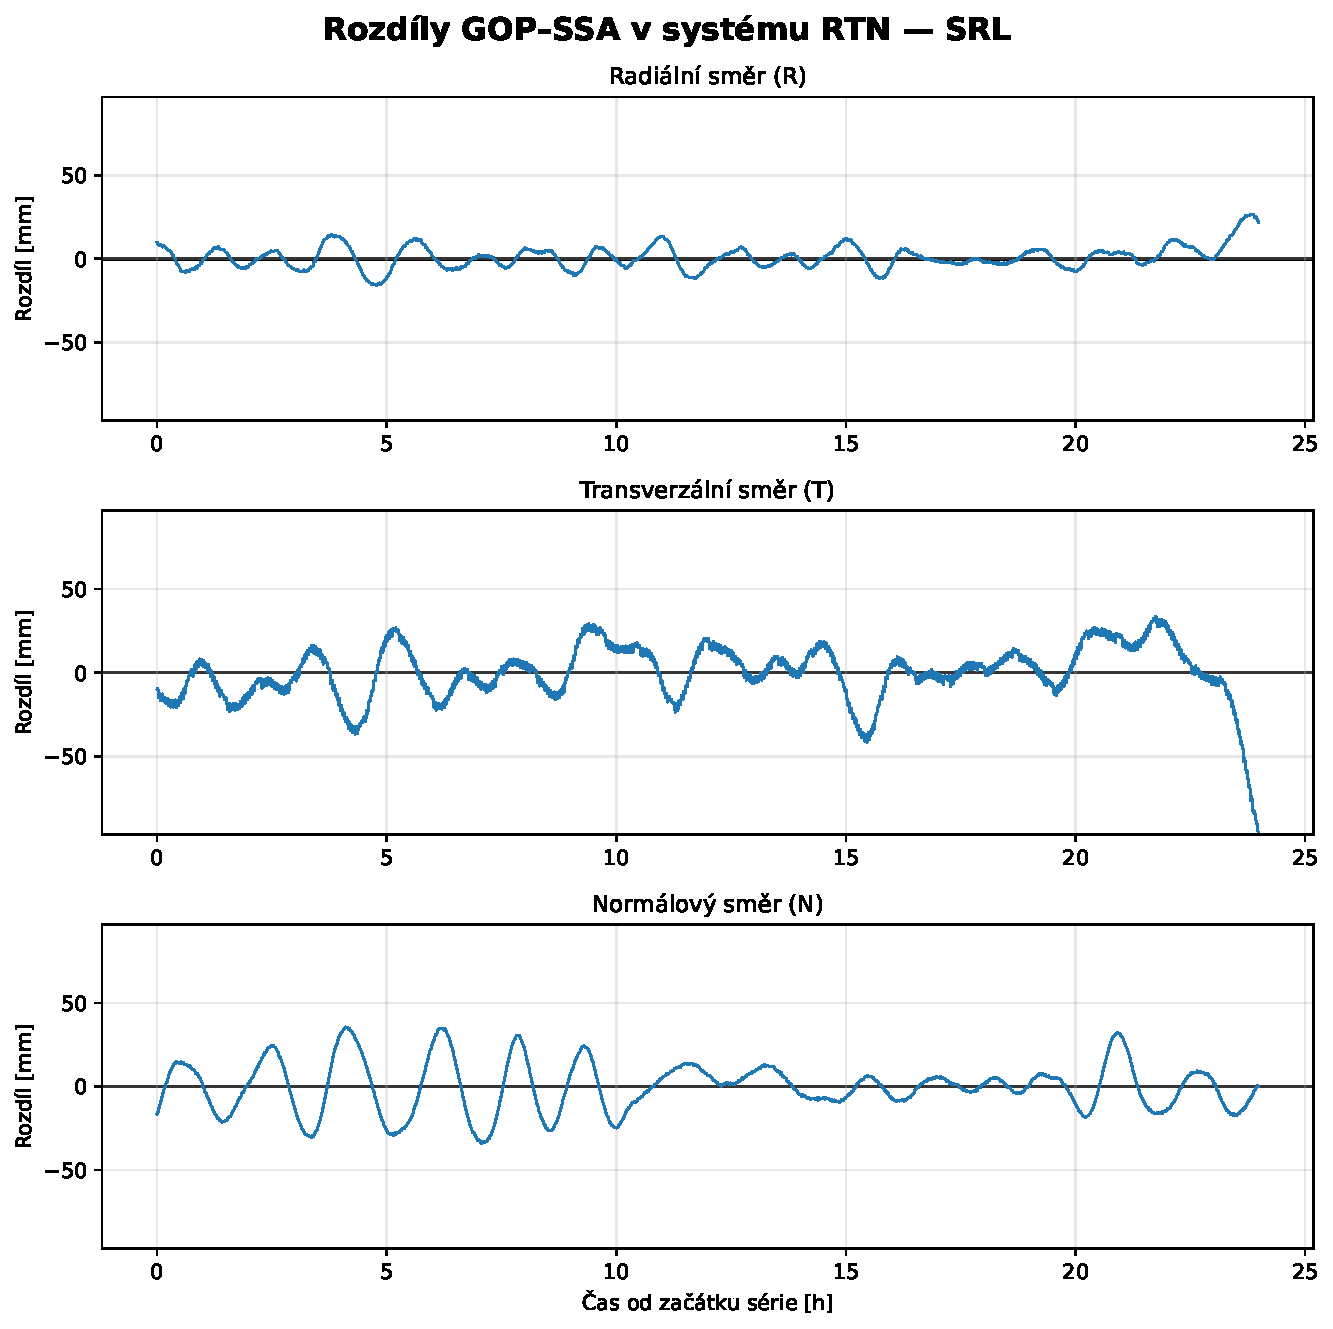
\includegraphics[width=1\textwidth]{images/results/satellites/hermite/srl/gop_vs_ssa_srl_doy001_rtn_differences.pdf}
    \caption{Průběh rozdílů \zk{GOP}\,--\,\zk{SSA} v~systému RTN družice SARAL}
    \label{fig:srl_herm_diff_doy001}
\end{figure}

Z~obrázku~\ref{fig:srl_herm_diff_doy001} je patrné, že rozdíly mezi řešeními se v~jednotlivých složkách chovají odlišně. Radiální složka~R se pohybuje přibližně v~rozmezí $\pm$\,20\,mm bez výraznějšího trendu v~průběhu dne. Transverzální složka~T dosahuje přibližně $\pm$\,40\,mm, avšak ke konci analyzovaného dne rozdíl mezi oběma řešeními výrazně narůstá. Normálová složka~N vykazuje odchylky přibližně $\pm$\,50\,mm a~její průběh vykazuje známky systematické struktury.

Pro posouzení rozložení rozdílů jsou na~obrázku~\ref{fig:srl_herm_hist_doy001} uvedeny histogramy pro jednotlivé složky systému \zk{RTN}.

\begin{figure}[H]
    \centering
    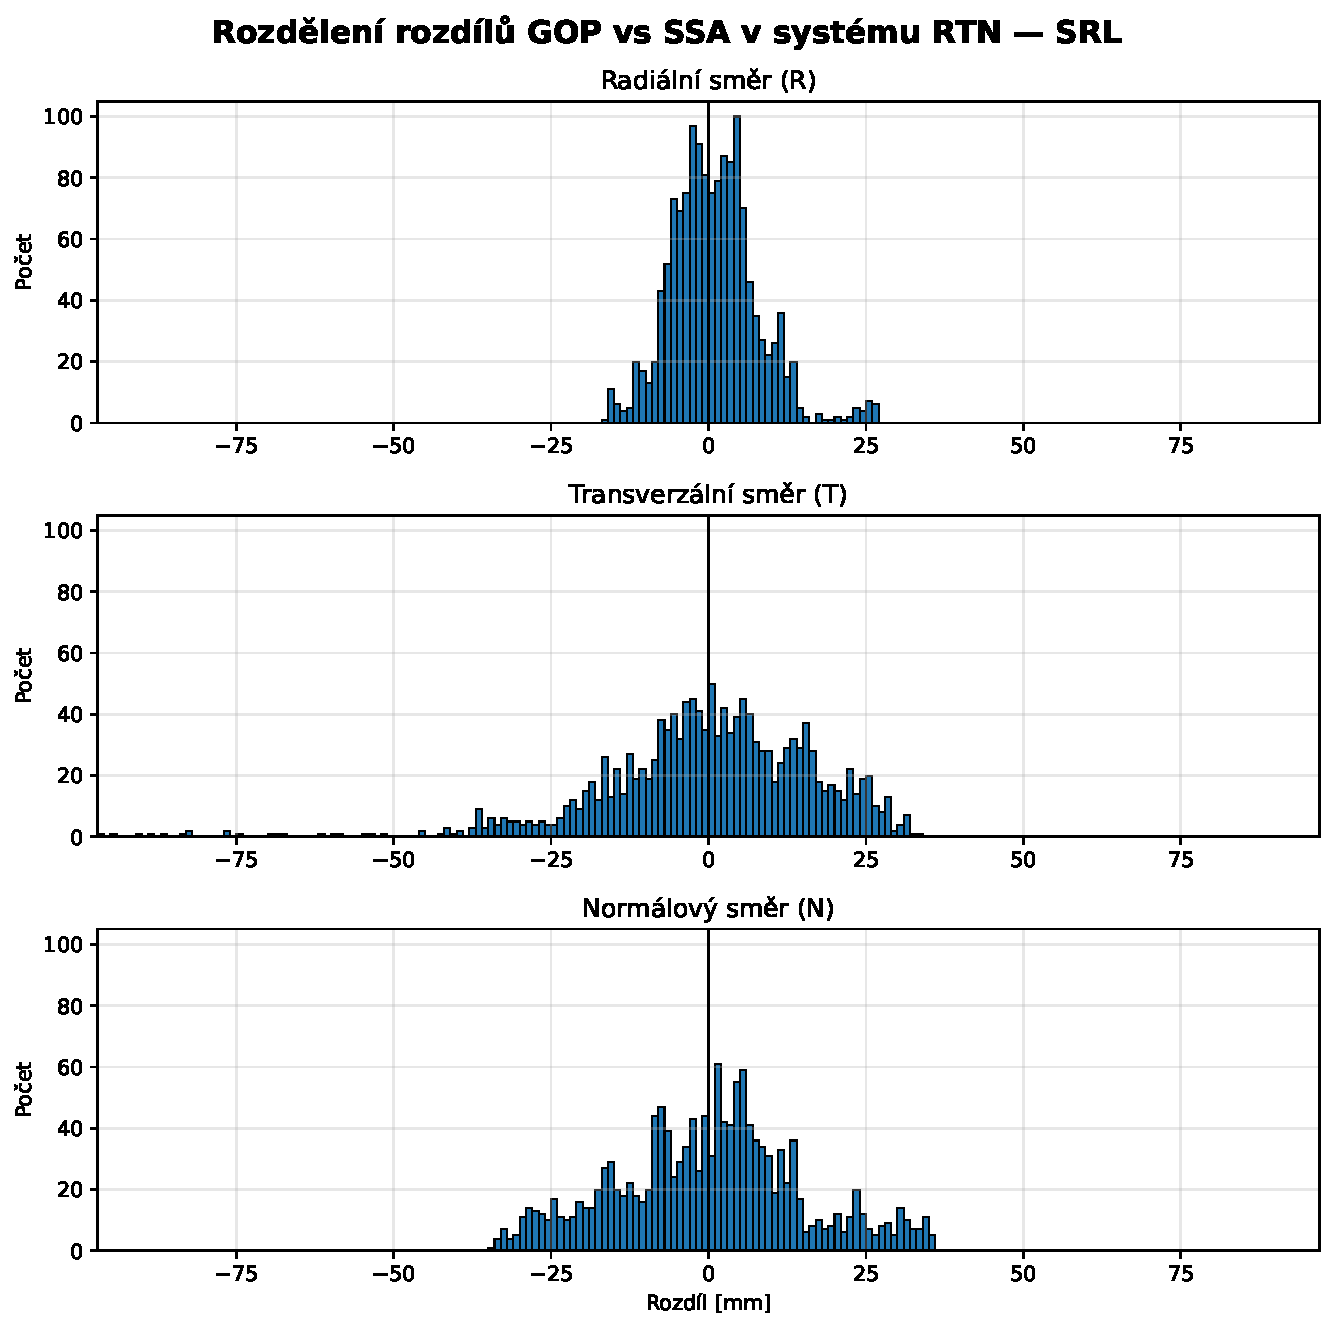
\includegraphics[width=1\textwidth]{images/results/satellites/hermite/srl/gop_vs_ssa_srl_doy001_rtn_histogram.pdf}
    \caption{Histogramy rozdílů \zk{GOP}\,--\,\zk{SSA} v~systému \zk{RTN} družice SARAL}
    \label{fig:srl_herm_hist_doy001}
\end{figure}

Z~histogramů vyplývá, že rozdíly jsou ve všech složkách soustředěny kolem nulové hodnoty a~není patrný výrazný systematický posun mezi oběma řešeními. Rozdělení se v~jednotlivých složkách liší šířkou i~tvarem. Radiální složka~R vykazuje nejužší a~nejsymetričtější rozdělení. Transverzální složka~T je výrazně širší a~mírně asymetrická s~přesahem do~záporných hodnot, který odpovídá nárůstu rozdílů ke konci analyzovaného dne. Normálová složka~N má plošší a~rovnoměrnější rozdělení, což odpovídá většímu rozptylu.

\paragraph{Spektrální analýza rozdílů}\leavevmode\\
Pro identifikaci periodicit v~rozdílech obou řešení byl vypočten Lomb--Scargleův periodogram, přičemž na~obrázku~\ref{fig:srl_herm_pg_doy001} jsou znázorněny periodogramy pro jednotlivé složky systému \zk{RTN}.

\begin{figure}[H]
    \centering
    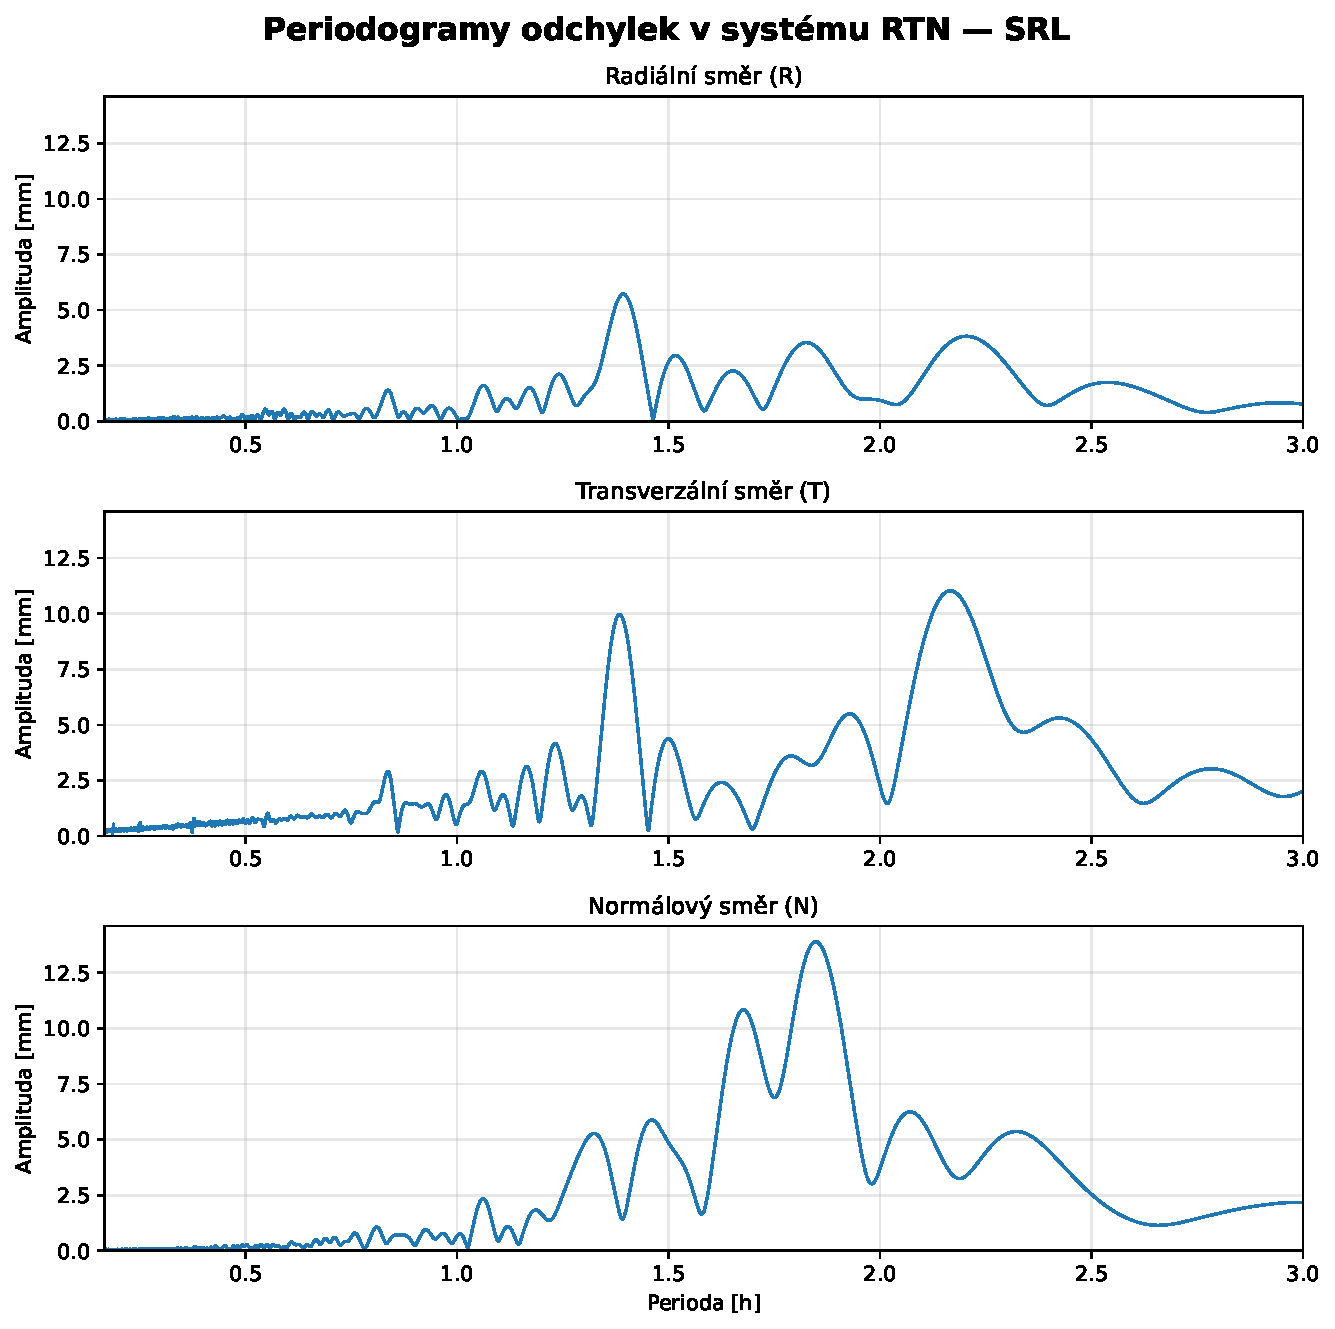
\includegraphics[width=1\textwidth]{images/results/satellites/hermite/srl/gop_vs_ssa_srl_doy001_rtn_periodograms_lomb_scargle.pdf}
    \caption{Periodogram rozdílů \zk{GOP}\,--\,\zk{SSA} v~systému \zk{RTN} družice SARAL}
    \label{fig:srl_herm_pg_doy001}
\end{figure}

Z~periodogramů je patrné, že v~normálové složce~N jsou přítomny výrazné vrcholy v~oblasti period přibližně 80--110\,min, tedy v~okolí oběžné doby družice \zkratka{SARAL}. Podobné vrcholy jsou patrné také v~transverzální složce~T, zatímco v~radiální složce~R jsou amplitudy výrazně nižší.

\paragraph{Dlouhodobá stabilita rozdílů}\leavevmode\\
Pro posouzení časové stability jsou na~obrázku~\ref{fig:srl_herm_rms_daily} znázorněny denní hodnoty \zkratka{RMS} rozdílů ve složkách \zk{RTN} a~celkové 3D~\zkratka{RMS} v~průběhu prvních 30~dnů roku 2024.

\begin{figure}[H]
    \centering
    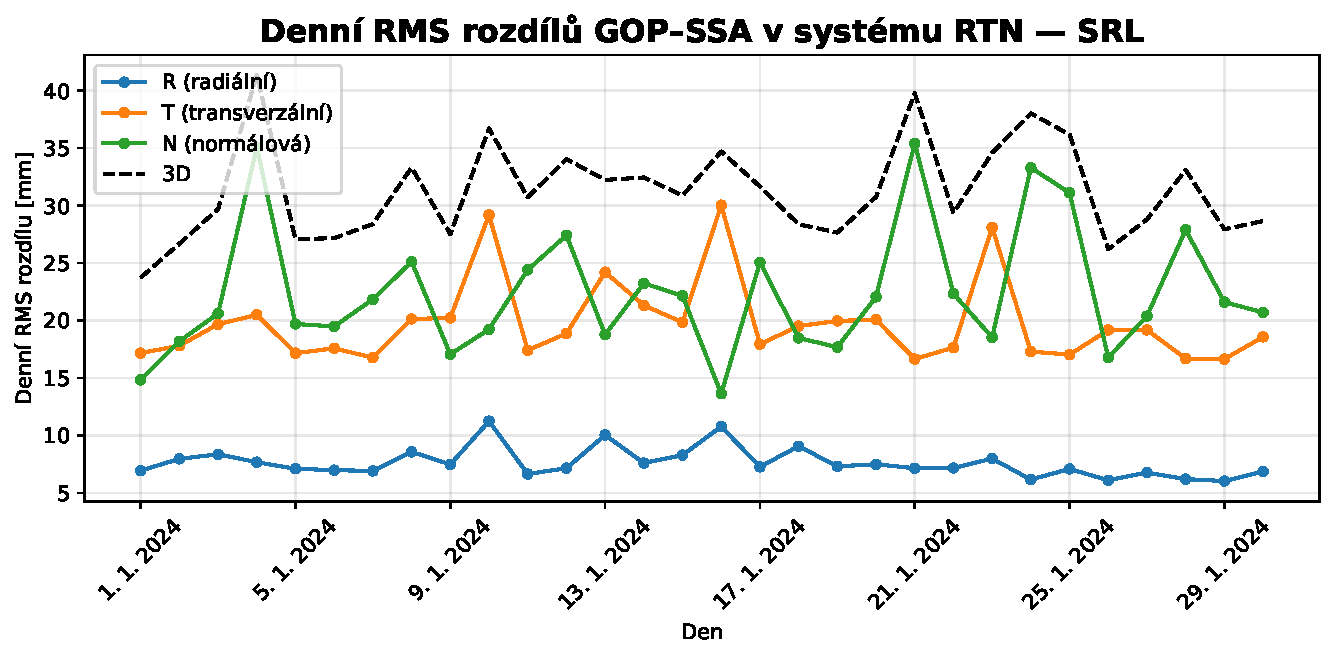
\includegraphics[width=1\textwidth]{images/results/satellites/hermite/srl/gop_vs_ssa_srl_doy001-doy030_daily_rtn_3d_rms.pdf}
    \caption{Denní RMS rozdílů \zk{GOP}\,--\,\zk{SSA} získané Hermitovou interpolací}
    \label{fig:srl_herm_rms_daily}
\end{figure}

Z~grafu je patrné, že hodnoty \zkratka{RMS} v~radiální složce jsou v~celém analyzovaném období stabilní a~pohybují se přibližně v~rozmezí 6--11\,mm, průměrně kolem 8\,mm. Transverzální složka~T dosahuje hodnot zhruba 16--30\,mm (průměrně $\sim$20\,mm), zatímco normálová složka~N se pohybuje v~rozsahu 14--35\,mm (průměrně $\sim$25\,mm) a~vykazuje největší variabilitu mezi jednotlivými dny. Celkové 3D~\zkratka{RMS} se pohybuje průměrně kolem 33\,mm.

\subsubsection{Porovnání pomocí dynamické parametrizace}

Druhý přístup vychází z~dynamické parametrizace v~\zkratka{BSW}. Dráhy ve formátu SP3 jsou v~modulu \texttt{ORBGEN} využity k~získání dynamické reprezentace dráhy. Rozdíly jsou určeny jako rozdíly polohy těchto drah ve společných epochách.

\paragraph{Průběh rozdílů v~rámci jednoho dne}\leavevmode\\
Na obrázku~\ref{fig:srl_bsw_diff_doy001} je znázorněn průběh rozdílů \zk{GOP}\,--\,\zk{SSA} ve složkách \zk{RTN} získaných pomocí dynamické parametrizace v~softwaru \zkratka{BSW}.

\begin{figure}[H]
    \centering
    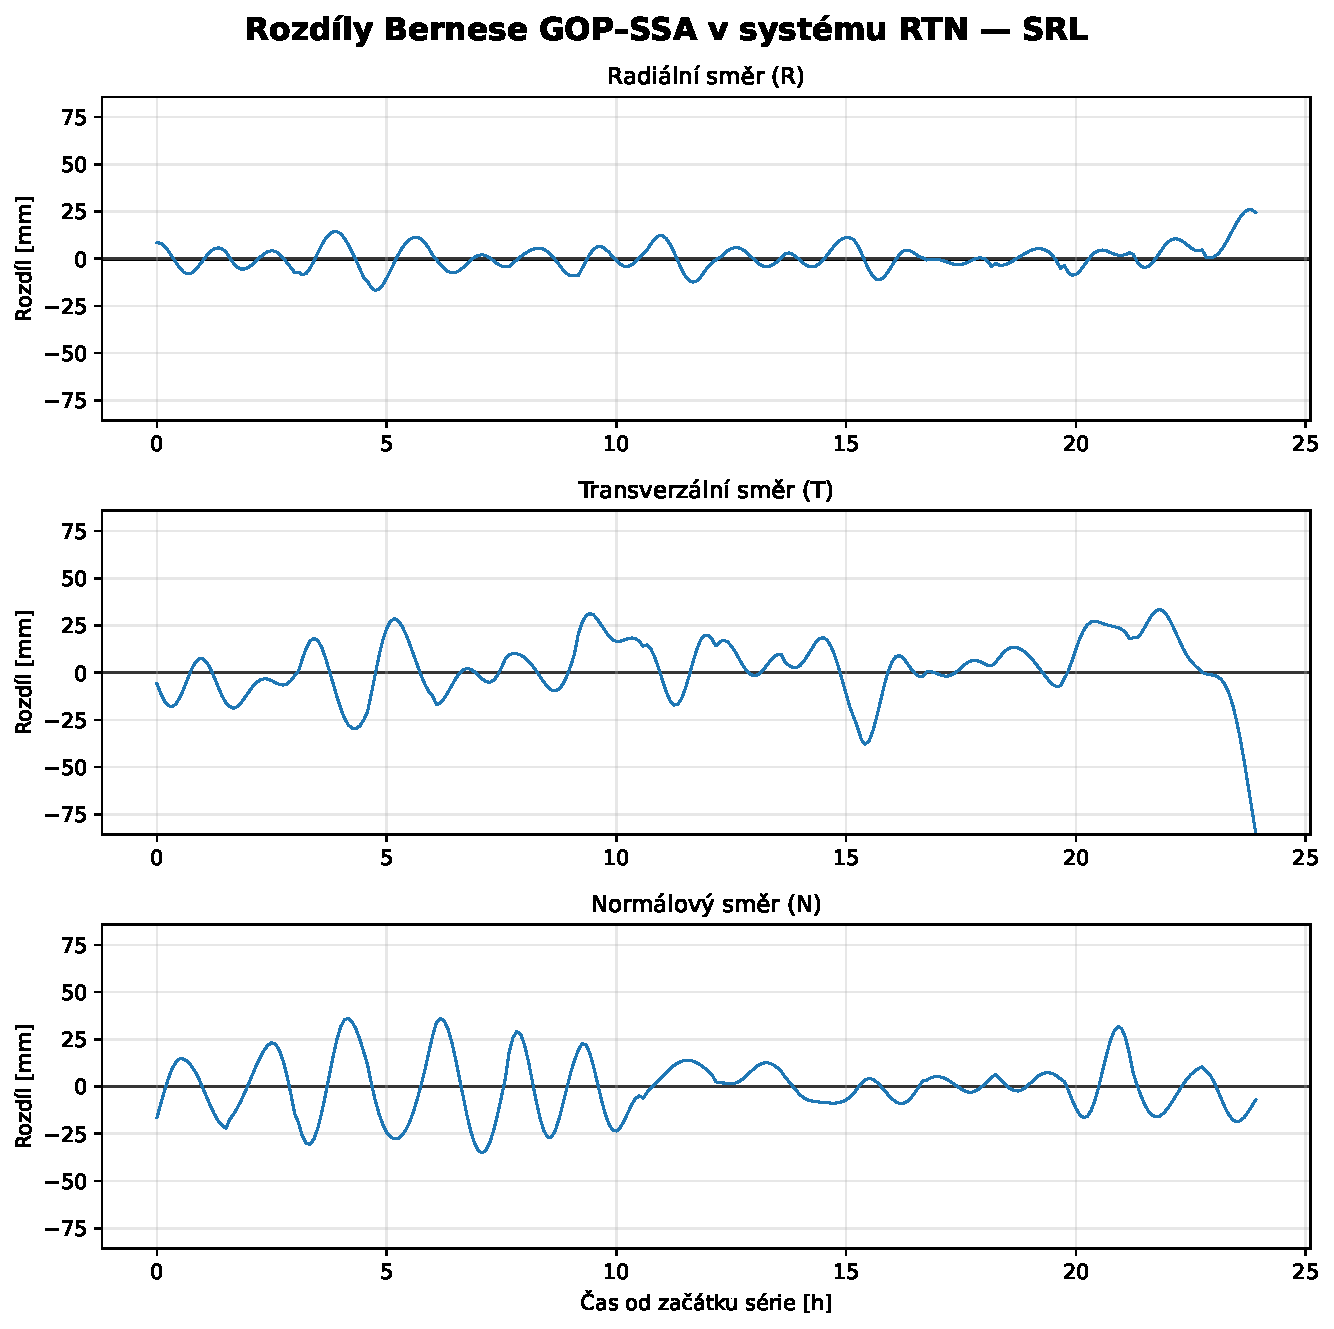
\includegraphics[width=1\textwidth]{images/results/satellites/bernese/sa/sa_ZAZG_doy001_rtn_differences.pdf}
    \caption{Průběh rozdílů \zk{GOP}\,--\,\zk{SSA} získaných dynamickou parametrizací}
    \label{fig:srl_bsw_diff_doy001}
\end{figure}

Průběh rozdílů je ve všech třech složkách prakticky totožný s~výsledky Hermitovy interpolace. Histogramy a~periodogram rozdílů jsou téměř shodné s~výsledky interpolační metody a~jsou uvedeny v~příloze.

\paragraph{Stabilita rozdílů v~čase}\leavevmode\\
Na obrázku~\ref{fig:srl_bsw_rms_daily} jsou znázorněny denní hodnoty \zkratka{RMS} rozdílů \zk{GOP}\,--\,\zk{SSA} ve složkách \zk{RTN} a~celkové 3D~\zkratka{RMS} v~průběhu prvních 30~dní roku 2024.

\begin{figure}[H]
    \centering
    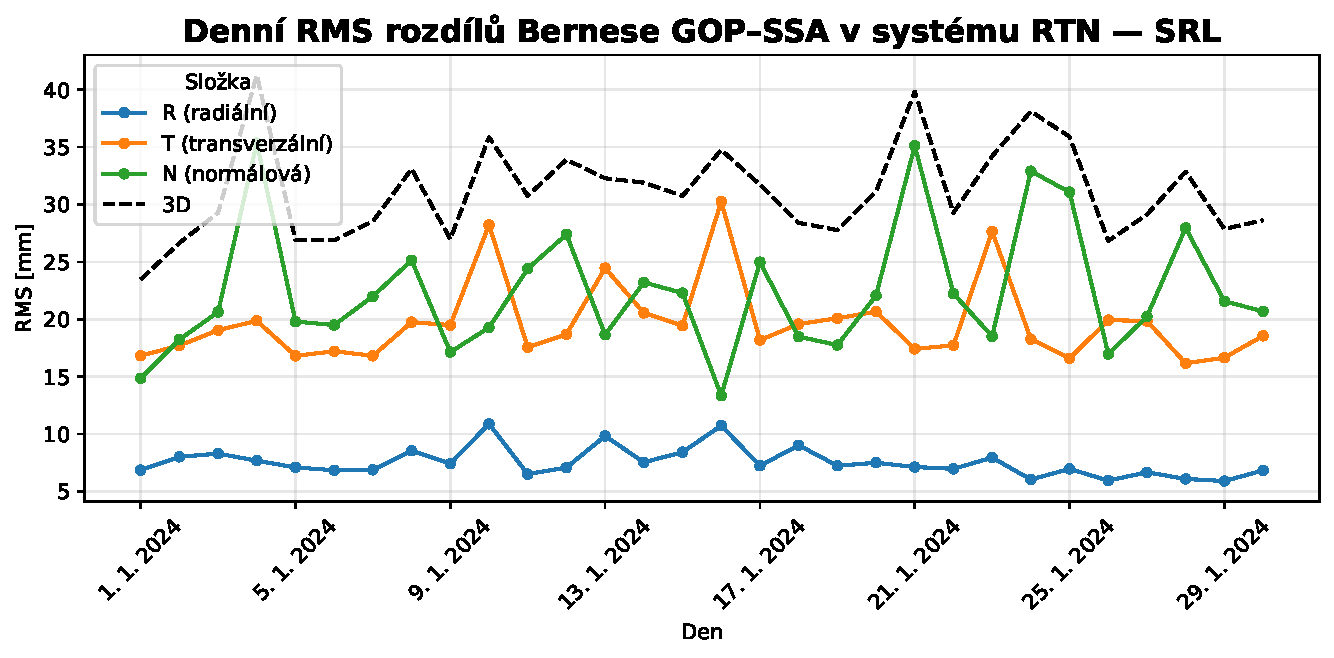
\includegraphics[width=1\textwidth]{images/results/satellites/bernese/sa/sa_ZAZG_doy001-doy030_daily_rtn_3d_rms.pdf}
    \caption{Denní RMS rozdílů \zk{GOP}\,--\,\zk{SSA} získané dynamickou parametrizací}
    \label{fig:srl_bsw_rms_daily}
\end{figure}

Hodnoty jsou prakticky totožné s~výsledky Hermitovy interpolace.

\subsubsection{Srovnání obou přístupů}

Pro přímé srovnání obou metod jsou na~obrázku~\ref{fig:srl_comp_overlay} vykresleny \zk{RTN} rozdíly získané interpolační metodou (modře) a~dynamickou parametrizací (oranžově).

\begin{figure}[H]
    \centering
    
\includegraphics[width=1\textwidth]{images/results/satellites/comparison/srl/hermite_vs_bernese_doy001_rtn_overlay.pdf}
    \caption{Porovnání RTN rozdílů \zk{GOP}\,--\,\zk{SSA} získaných interpolací a parametrizací}
    \label{fig:srl_comp_overlay}
\end{figure}

Z~obrázku je patrné, že obě metody poskytují v~celém průběhu prakticky totožné výsledky ve všech třech složkách \zk{RTN}. Vzájemné odchylky se pohybují na~úrovni jednotek milimetrů, přičemž průběh získaný dynamickou parametrizací je ve srovnání s~interpolační metodou mírně vyhlazenější.

Shoda obou přístupů naznačuje, že pro porovnání přesných drah se vzorkováním 60\,s je Hermitova interpolace plnohodnotnou alternativou k~dynamické parametrizaci a~umožňuje získat srovnatelné výsledky bez nutnosti využití fyzikálního modelu a~softwaru \zkratka{BSW}.

\subsubsection{Interpretace}

Porovnání přesných drah \zk{GOP} a~\zk{SSA} pro družici \zkratka{SARAL} ukazuje, že obě řešení jsou vzájemně konzistentní bez výrazného systematického posunu. Radiální složka~R je nejstabilnější s~průměrnou hodnotou RMS přibližně 8\,mm. Transverzální složka~T dosahuje průměrně přibližně 20\,mm a~normálová složka~N vykazuje největší variabilitu v~rozsahu 14--35\,mm (průměrně $\sim$25\,mm). V~periodogramu jsou přítomny výrazné vrcholy v~oblasti oběžné doby družice \zkratka{SARAL} ($\sim$100\,min), a~to zejména ve složkách N a~T, což naznačuje, že část rozdílů mezi oběma řešeními souvisí s~oběžnou dobou družice. Shoda obou metod porovnání potvrzuje, že zjištěné rozdíly jsou vlastností samotných drahových řešení, nikoli artefaktem zvolené metody analýzy.

\subsection{Souhrnné výsledky}
\label{sec:souhrn-drahy}

Souhrnné hodnoty \zk{RMS} rozdílů drah \zk{GOP}\,--\,\zk{SSA} získané Hermitovou interpolací jsou uvedeny v~tabulce~\ref{tab:gop_vs_ssa_satellites_doy001-doy030_hermite_rms}.

\begin{table}[H]
\centering
\small
\caption{Průměrné RMS rozdílů GOP--SSA získané Hermitovou interpolací}
\label{tab:gop_vs_ssa_satellites_doy001-doy030_hermite_rms}
\begin{tabular}{lrrr}
\toprule
Družice & R [mm] & T [mm] & N [mm] \\
\midrule
SRL & 7.72 & 20.06 & 23.07 \\
CS2 & 9.03 & 26.10 & 24.88 \\
H2C & 9.81 & 28.54 & 37.39 \\
H2D & 8.40 & 33.09 & 28.19 \\
JA3 & 10.24 & 28.21 & 44.14 \\
S3A & 8.48 & 23.41 & 30.56 \\
S3B & 8.30 & 23.34 & 25.71 \\
S6A & 8.14 & 28.78 & 38.60 \\
\bottomrule
\end{tabular}
\end{table}

Dále jsou stručně shrnuty hlavní charakteristiky rozdílů drah pro jednotlivé analyzované družice.

\subsubsection{SARAL}

Rozdíly drah GOP a SSA jsou ve složce R stabilní v~celém analyzovaném období a~pohybují se přibližně v~rozmezí 6--11\,mm. Transverzální složka T dosahuje hodnot přibližně 17--30\,mm a~normálová složka N vykazuje největší variabilitu v~rozsahu přibližně 14--35\,mm. V~periodogramu normálové složky je přítomna dominantní periodicita v~oblasti oběžné doby družice. Obě použité metody -- Hermitova interpolace i~dynamická parametrizace v~softwaru \zkratka{BSW} -- poskytují srovnatelné výsledky s~rozdíly na~úrovni milimetrů.

\subsubsection{CryoSat-2}

CryoSat-2 vykazuje celkově stabilní rozdíly drah \zk{GOP}\,--\,\zk{SSA} v~celém analyzovaném období. Radiální složka R dosahuje hodnot RMS průměrně 8{,}9~mm s~rozsahem přibližně 7--12~mm. Transverzální složka T se pohybuje průměrně kolem 26~mm s~rozsahem přibližně 20--32~mm. Normálová složka N dosahuje průměrně přibližně 24~mm a~vykazuje největší variabilitu v~rozmezí přibližně 18--40~mm. Ke konci ledna 2024 byl ve složce N zaznamenán výraznější nárůst RMS na~hodnotu přibližně 40~mm. V~periodogramu normálové složky je přítomna periodicita odpovídající oběžné době družice ($\sim$99~min). Vzájemné odchylky Hermitovy interpolace a~dynamické parametrizace v~BSW se pohybují na~úrovni jednotek milimetrů.

\subsubsection{HY-2C}

HY-2C vykazuje v~rámci satelitů HY-2 zvýšenou variabilitu normálové složky N. Radiální složka R dosahuje průměrných hodnot RMS přibližně 10~mm s~rozsahem přibližně 6--18~mm. Transverzální složka T se pohybuje kolem 28~mm s~rozsahem přibližně 19--50~mm. Normálová složka N vykazuje největší variabilitu s~průměrnými hodnotami RMS kolem 36~mm a~rozsahem přibližně 15--56~mm. V~periodogramu normálové složky je přítomna dominantní periodicita odpovídající oběžné době družice ($\sim$104~min). Vzájemné odchylky Hermitovy interpolace a~dynamické parametrizace v~BSW se pohybují na~úrovni jednotek milimetrů.

\subsubsection{HY-2D}

HY-2D vykazuje v~průběhu analyzovaného období celkově stabilní rozdíly 
drah. Radiální složka R dosahuje hodnoty RMS průměrně 8{,}1~mm s~rozsahem 
5--17~mm. Transverzální složka T se pohybuje průměrně kolem 28~mm 
s~rozsahem 16--40~mm. V~denních hodnotách RMS byl dne 26.~1.~2024 
zaznamenán výjimečný nárůst na přibližně 100~mm, jehož původ nebyl 
jedno\-značně objasněn. Normálová složka N dosahuje průměrně přibližně 
27~mm s~rozsahem 17--53~mm. V~periodogramu je přítomna periodicita 
odpovídající oběžné době ($\sim$104~min). Vzájemné odchylky Hermitovy 
interpolace a~dynamické parametrizace v~BSW se pohybují na~úrovni 
jednotek milimetrů.

\subsubsection{Jason-3}

Jason-3 vykazuje ze všech analyzovaných satelitů nejvyšší variabilitu normálové složky N. Radiální složka R dosahuje průměrné hodnoty RMS přibližně 10~mm s~rozsahem 7--15~mm. Transverzální složka T se pohybuje průměrně kolem 28~mm s~rozsahem 19--38~mm. Normálová složka N dosahuje průměrné hodnoty RMS 41~mm s~rozsahem 12--84~mm. V~denních hodnotách RMS byl dne 3.~1.~2024 zaznamenán výrazný nárůst na přibližně 84~mm. V~periodogramu je přítomna periodicita odpovídající oběžné době ($\sim$112~min). Celkový charakter rozdílů je analogický k~družici Sentinel-6A, se kterou sdílí orbitální výšku ($\sim$1\,336~km). Vzájemné odchylky Hermitovy interpolace a~dynamické parametrizace v~BSW se pohybují na~úrovni jednotek milimetrů.

\subsubsection{Sentinel-3A}

Sentinel-3A vykazuje stabilní rozdíly drah \zk{GOP}\,--\,\zk{SSA} po celé analyzované 
období. Radiální složka R dosahuje průměrné hodnoty RMS přibližně 8~mm 
s~rozsahem 5--12~mm. Transverzální složka T se pohybuje průměrně kolem 
23~mm s~rozsahem 17--36~mm. Normálová složka N dosahuje průměrné hodnoty 
RMS přibližně 29~mm s~rozsahem 15--52~mm. V~denních hodnotách RMS byl 
kolem 16.~1.~2024 zaznamenán výraznější nárůst na přibližně 52~mm. 
V~periodogramu je přítomna periodicita odpovídající oběžné době 
($\sim$101~min). Výsledky jsou velmi podobné sesterské družici Sentinel-3B, 
což odpovídá totožné orbitální výšce obou satelitů. Vzájemné odchylky 
Hermitovy interpolace a~dynamické parametrizace v~BSW se pohybují 
na~úrovni jednotek milimetrů.

\subsubsection{Sentinel-3B}

Sentinel-3B vykazuje stabilní rozdíly drah \zk{GOP}\,--\,\zk{SSA} velmi podobné 
sesterské družici Sentinel-3A, což odpovídá totožné orbitální výšce 
obou satelitů. Radiální složka R dosahuje průměrné hodnoty RMS přibližně 
8~mm s~rozsahem 6--14~mm. Transverzální složka T se pohybuje průměrně 
kolem 23~mm s~rozsahem 18--37~mm. Normálová složka N dosahuje průměrné 
hodnoty RMS přibližně 25~mm s~rozsahem 14--47~mm. V~denních hodnotách 
RMS byl kolem 25.~1.~2024 zaznamenán výraznější nárůst na přibližně 
47~mm. V~periodogramu je přítomna periodicita odpovídající oběžné době 
($\sim$101~min). Vzájemné odchylky Hermitovy interpolace a~dynamické 
parametrizace v~BSW se pohybují na~úrovni jednotek milimetrů.

\subsubsection{Sentinel-6A}

Sentinel-6A vykazuje vysokou variabilitu normálové složky N analogicky k~družici Jason-3, se kterou sdílí podobnou orbitální výšku ($\sim$1\,336~km). Radiální složka R dosahuje průměrných hodnot RMS přibližně 8~mm s~rozsahem přibližně 5--12~mm. Transverzální složka T se pohybuje kolem 29~mm s~rozsahem přibližně 20--38~mm. Normálová složka N dosahuje průměrných hodnot RMS přibližně 37~mm a~vykazuje největší variabilitu v~rozmezí přibližně 18--79~mm. Dne 11.~1.~2024 byl ve složce N zaznamenán výrazný nárůst RMS na~hodnotu přibližně 79~mm. V~periodogramu jsou přítomny výrazné vrcholy ve složkách N a~T s~dominantní periodicitou v~oblasti oběžné doby družice ($\sim$112~min). Vzájemné odchylky Hermitovy interpolace a~dynamické parametrizace v~BSW se pohybují na~úrovni jednotek milimetrů.